% % part: 支持向量机
% % chapter: 基本支持向量机

% \documentclass[UTF8]{ctexbook}

% \ctexset{
%     part/number = \chinese{part}
% }
% \usepackage{multirow}
% \usepackage{amsmath}% ams 数学公式
% \usepackage{amsfonts}% ams 数学字体
% \usepackage{bbm}%重影字体
% \usepackage{amssymb,latexsym}% ams 数学符号与LaTeX数学符号
% \usepackage{mathrsfs}% 花式符号
% \usepackage{ntheorem}%定理、定义、证明
%     \theoremstyle{nonumberplain}
%     \theoremheaderfont{\bfseries}
%     \theorembodyfont{\normalfont}
%     \theoremsymbol{$\square$}
%     \newtheorem{Proof}{\hskip 2em 证明}
%     \newtheorem{theorem}{\hspace{2em}定理}[chapter]
%     \newtheorem{definition}{\hspace{2em}定义}[chapter] % 如果没有章, 只有节, 把上面的[chapter]改成[section]
%     \newtheorem{axiom}[definition]{\hspace{2em}公理}
%     \newtheorem{lemma}[definition]{\hspace{2em}引理}
%     \newtheorem{proposition}[definition]{\hspace{2em}命题}
%     \newtheorem{corollary}[definition]{\hspace{2em}推论}
%     \newtheorem{remark}{\hspace{2em}注}[chapter] %类似地定义其他“题头”. 这里“注”的编号与定义、定理等是分开的
%     \newtheorem{Assumption}{\hspace{2em}假设}[chapter]

% %算法伪代码
% %http://blog.csdn.net/lwb102063/article/details/53046265
% \usepackage{algorithm}
% \usepackage{algorithmicx}
% \usepackage{algpseudocode}
%     \floatname{algorithm}{算法}
%     \renewcommand{\algorithmicrequire}{\textbf{输入:}}
%     \renewcommand{\algorithmicensure}{\textbf{输出:}}
% % 罗马数字:示例:\rom{2}
% \makeatletter
% \newcommand*{\rom}[1]{\expandafter\@slowromancap\romannumeral #1@}
% \makeatother

% \usepackage{enumerate}%itemiz环境。\begin{enumerate}[step 1][a)]可以使用 A,a,I,i,1 作为可选项产生 \Alph,\alph,\Roman,\roman,\arabic 的效果
% \usepackage{cite}%参考文献
%     \bibliographystyle{plain}
% \usepackage{extarrows}% 带参数的箭头
% \usepackage{hyperref}% 超链接
% \usepackage{pifont}%然后在正文输入\ding{172}~\ding{211}得到相应数字,要是要①就输入:\ding{172}②就输:\ding{173}
% %\usepackage[CJKbookmarks, colorlinks, bookmarksnumbered=true,pdfstartview=FitH,linkcolor=black,citecolor=black]{hyperref}%超链接的格式设置
% \hypersetup{
%     colorlinks=false,% 去掉超链接颜色
%     pdfborder=0 0 0% 取消超链接的边框
% }
% \usepackage{graphicx}% 图片管理
% \usepackage{caption}
% \usepackage{subcaption}%并排的图各有标题
% \graphicspath{{images/}}% 设置图片搜索路径
% \usepackage{float,varwidth}% 浮动体
% \usepackage{booktabs}% 三线表
% \usepackage{fancyhdr}% 页眉设置
% \usepackage{xcolor}% 颜色宏包
% \usepackage{colortbl}% 彩色表格
% \usepackage{listings}% 代码高亮
% \usepackage{caption}% 对标题进行控制,如让\caption标题的字体缩小一号,同时数字标签使用粗体可以用:\usepackage[font=small,labelfont=bf]{caption}
% \usepackage{xfrac,upgreek}%分别是行间公式如a/b的形式(将原来的命令\frac改成\sfrac)和希腊字体的宏包的
% \usepackage{mathtools}%lgathered和rgathered环境把公式向左向右对齐
% \usepackage{tabularx}%提供自动延伸的表列,(X列格式说明符),文字过长时可以自动转行
% \usepackage{longtable}%长表格
% \usepackage{enumitem}%enumerate宏包的升级
% \usepackage{harpoon}%数学公式的矢量
% \usepackage{bookmark}%目录的书签
% \renewcommand{\headwidth}{\textwidth}%图片并排,这个要列在所有宏包的后面
% \definecolor{codegreen}{rgb}{0,0.6,0}
% \definecolor{codegray}{rgb}{0.5,0.5,0.5}
% \definecolor{codepurple}{rgb}{0.58,0,0.82}
% \definecolor{backcolour}{rgb}{0.95,0.95,0.92}
% \lstset{
%     commentstyle=\color{codegreen},
%     keywordstyle=\color{magenta},
%     numberstyle=\tiny\color{codegray},
%     stringstyle=\color{codepurple},
%     basicstyle=\footnotesize,
%     breakatwhitespace=false,% 断行只在空格处
%     breaklines=true,% 自动断行
%     captionpos=b,% 标题位置
%     keepspaces=true,
%     numbers=left,
%     numbersep=5pt,
%     showspaces=false,
%     showstringspaces=false,
%     showtabs=false,% 显示
%     tabsize=2% TAB 被当作两个空格
% }
% \topmargin=0pt\oddsidemargin=0pt\evensidemargin=0pt
% \textwidth=16.5cm\textheight=23cm\raggedbottom%我这么设置是为了缩小页边距,满足有的文字无法转行
% \pagestyle{headings}%页眉为章节标题,无页脚
% \setlength{\abovecaptionskip}{10pt}
% \setlength{\belowcaptionskip}{-15pt}%图片表格的前后距离设置
% \CTEXsetup[format={\zihao{-3}\raggedright\bfseries}]{section}%设置节的格式

% \begin{document}

% \part{支持向量机}
\chapter{基本支持向量机}
\section{支持向量机简介}
	% \label{sec:支持向量机-基本支持向量机-支持向量机简介}
	支持向量机(Support Vector Machine,SVM)由Corinna Cortes和Vapnik等人于1995年首先提出,最初被用于解决二分类问题。它在解决小样本、非线性及高维模式识别中表现出许多特有的优势,被广泛的应用于各种机器学习问题当中。

\section{支持向量机的引入}
	% \label{sec:支持向量机-基本支持向量机-支持向量机的引入}
	考虑这样一个二分类问题:特征变量(输入变量)是二维的,且总体类型只有两类,类别标签为$(-1,+1)$,其数据如表(\ref{tab:SVM模拟数据})所示
	\begin{table}[htbp]
		\caption{模拟数据}
		\label{tab:SVM模拟数据}
		\centering
		\begin{tabular}{l|lll}
		\toprule
		data   & $x_1$    & $x_2$    & $y$ \\
		\midrule
		1      & 2      & 2      & 1 \\
		2      & 3      & 1      & 1 \\
		3      & 2      & 0      & -1 \\
		$\vdots$ & $\vdots$ & $\vdots$ & $\vdots$ \\
		m      & $\cdot$  & $\cdot$  & $\cdot$ \\
		\bottomrule
		\end{tabular}
	\end{table}
	\par
	我们用$X=(x_1,x_2)\subset R^2$表示特征空间,$y$为样本类别,$y$的具体取值为标签值,例如:第$k$个样本的标签值为$y^k=1$。事实上,样本类别与样本的标签值无关,即(-1,+1)可以改为(0,+1),这并不影响类的本质,值得一提的是:后面介绍的某些方法(如SVM,logistics regression 等),其建模方法是依赖于标签值的。假设共有$m$个样本,用$x^k(k=1,2,...,m)$表示第$k$个样本的特征值,$x^k\in R^2$,例如:第一个样本的特征值写为$x^1=(3,2)$。我们可以将整个数据放在集合中,记为$S=\{x^k,y^k\}_{k=1}^m$。现在的问题是:找一个分类器$y=f(x)$,使它能够很好的将样本分开,并且由它得到的错误率等指标又可以接受。
	\par
	我们用一个图形来表示上面的问题,如图(\ref{fig:二分类问题示意图})所示
		\begin{figure}[H]
		\centering
		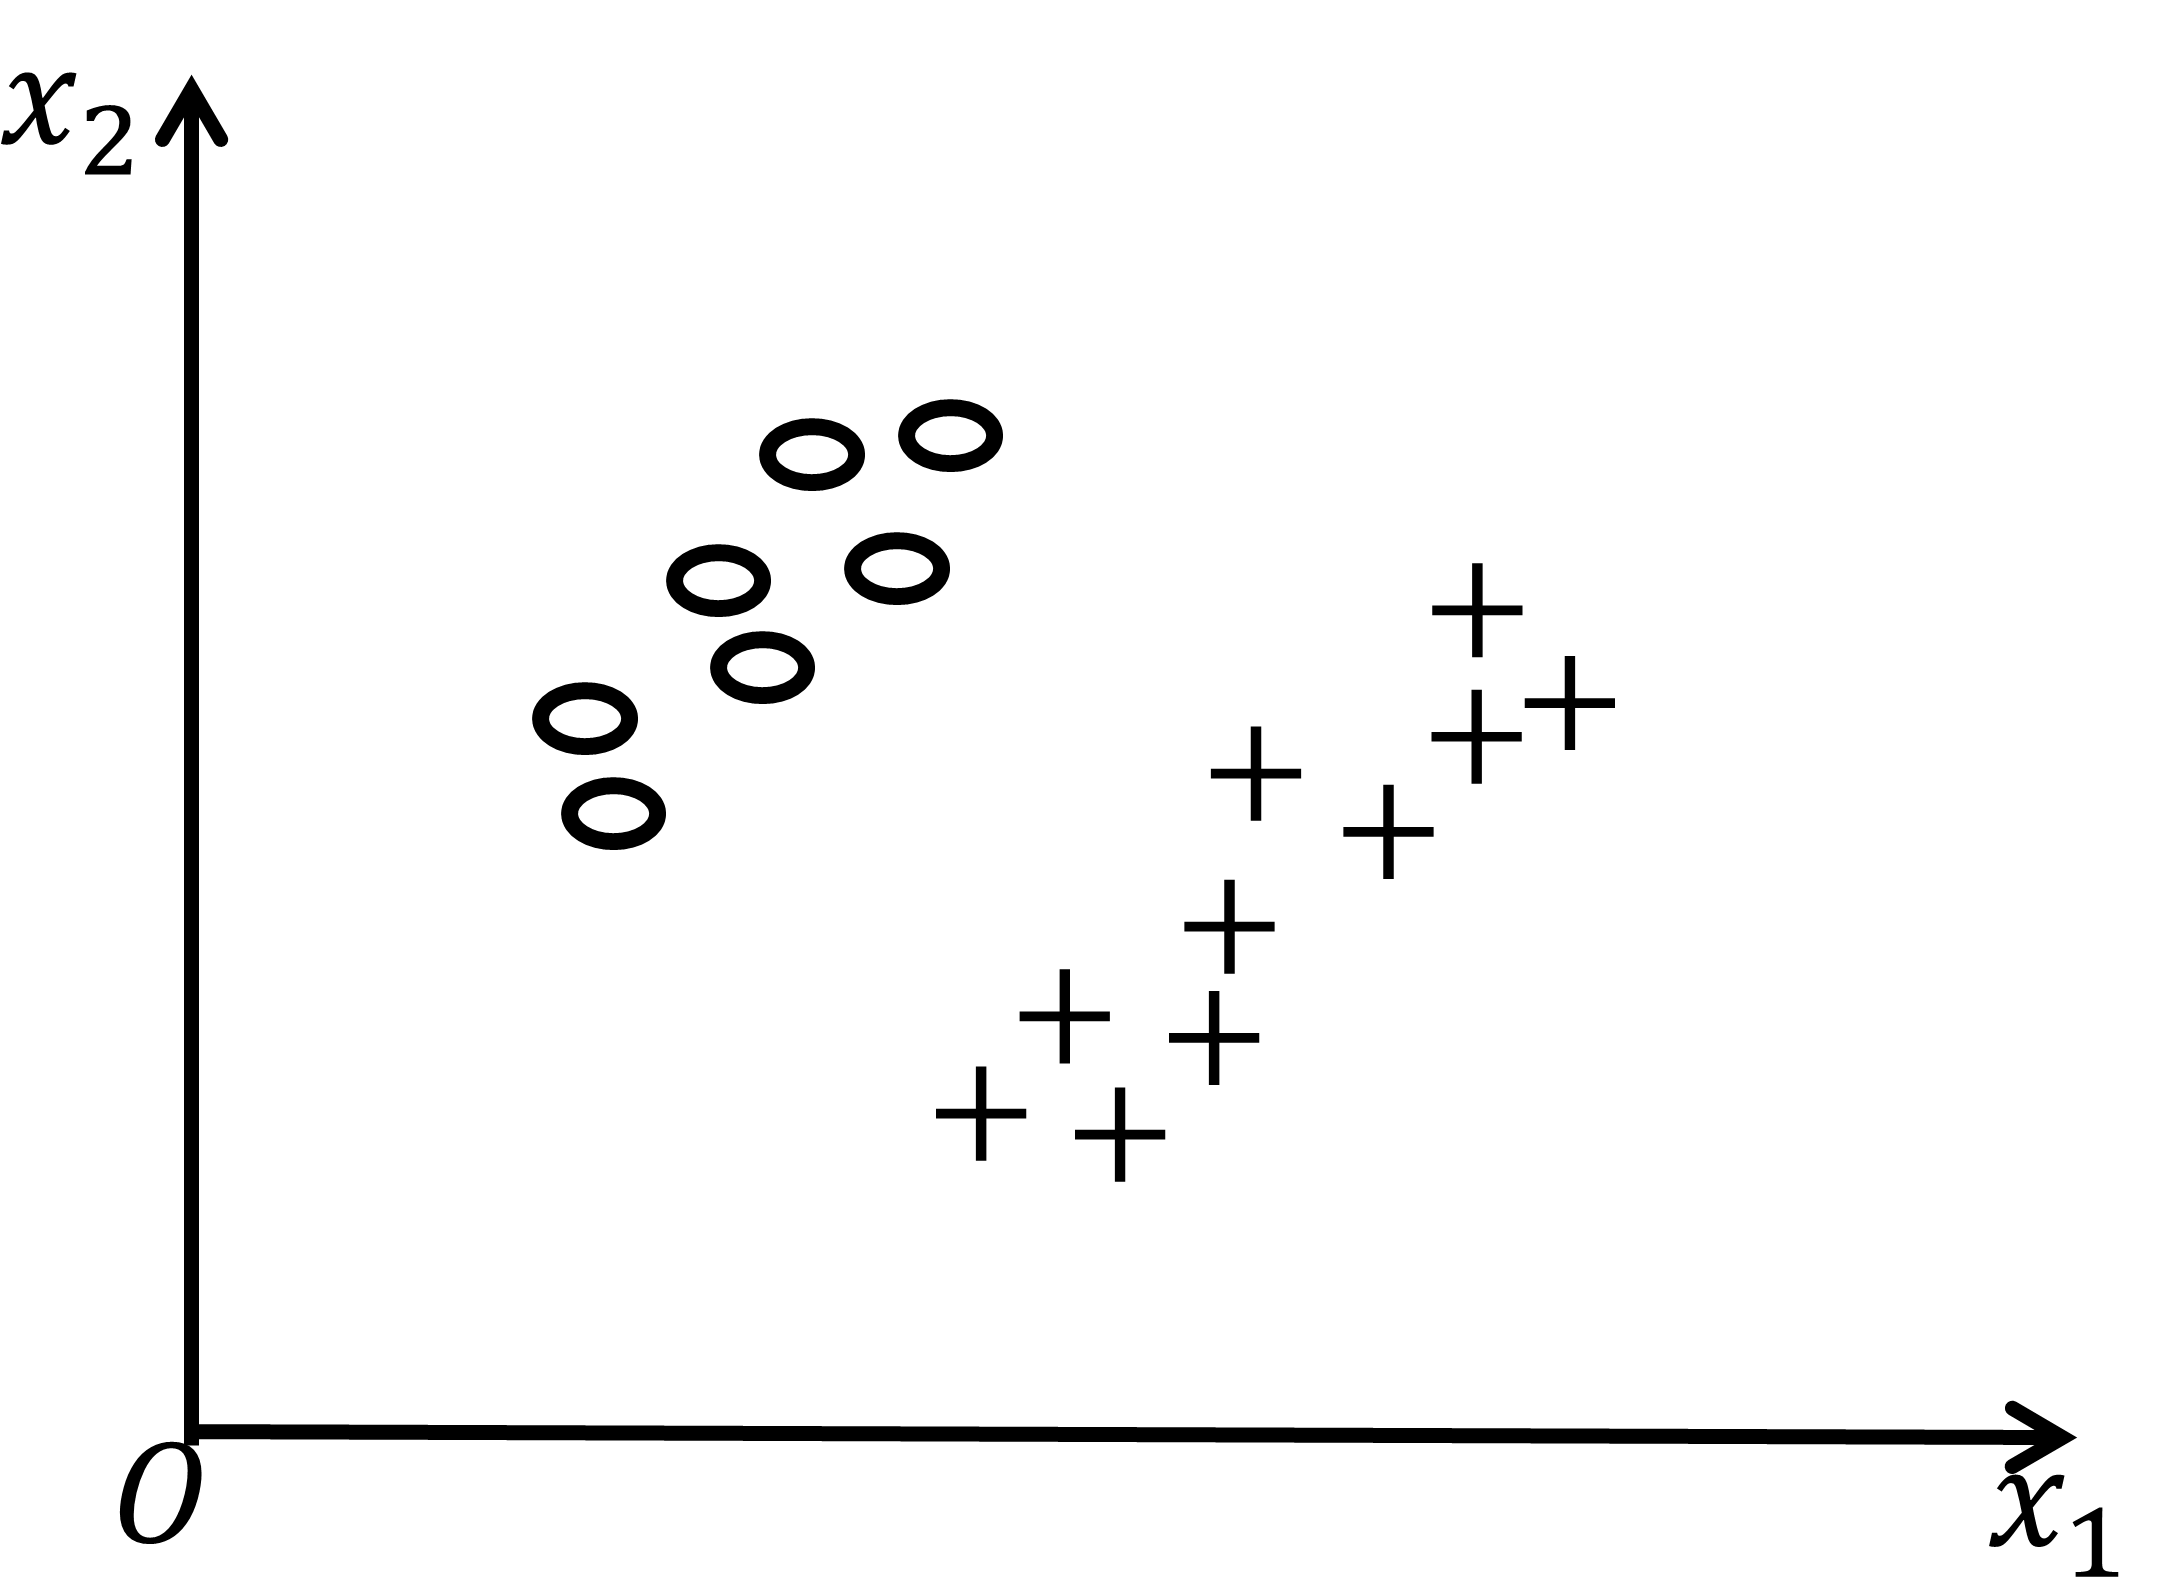
\includegraphics[width=4cm]{images/SVM_BSVM_classify_of_two.jpg}
		\caption{二分类问题示意图}
		\label{fig:二分类问题示意图}
		\end{figure}
	假设样本是线性可分的,我们用$\oplus$来表示$y=+1$,用$\ominus$来表示$y=-1$,每个样本即为图中的一个点,那么这个二分类问题就变为如何找到一条分割线(这里仅考虑直线),将$\oplus$和$\ominus$ 分割开。在这个$x_1Ox_2$平面直角坐标系中,任意一条直线将表示成$x_2=ax_1+b$,也即$w_1x_1+w_2x_2+b=0$ ,从直线表达式可以看出,只要确定了直线中的参数$(\mathbf w,b)$,直线也就确定了。所以,现在我们要思考的问题是:我们依据什么样的准则来确定直线参数?这里我们提出以下几种准则:
	\begin{enumerate}
	    \item 在参数$(\mathbf w,b)$的空间$\Theta$中,取$\mathbf w,b$使得两个群体点到直线的平均距离最大。
	    \item 在$\mathbf w,b\in \Theta$空间中,取$\mathbf w,b$使得两个群体到直线的平均距离最大。
	    \item 在$\mathbf w,b\in \Theta$空间中,取$\mathbf w,b$ 使得两个群体的中点到直线的距离最大。
	    \item 在$\mathbf w,b\in \Theta$空间中,取$\mathbf w,b$使得两个群体距离直线最近的点的距离最大。
	\end{enumerate}
	\par
	当然,还有其它一些准则可以使用,我们姑且记准则集合为$\pounds$。为了求直线,我们需要知道点到直线的距离,对平面上的某点$x^k=(x_1^k,x_2^k)$,其到直线$w_1x_1+w_2x_2+b=0$的距离$d$为
	\[
	d=\frac{| w_1x_1^k+w_2x_2^k+b| }{\|\mathbf w\|} = \frac{| w_1x_1^k+w_2x_2^k+b| }{\sqrt {w_1^2+w_2^2}}
	\]
	其中:$\|\mathbf w\|$为$\mathbf w=(w_1,w_2)$的$L_2$范数。并且如果$w_1x_1^k+w_2x_2^k+b>0$,则数据点$x^k$位于直线上方;如果$w_1x_1^k+w_2x_2^k+b<0$,则数据点位于直线下方。平面上一条直线将平面分为两部分($y=\pm 1$)。
	\par
	下面,我们在支持向量机的准则$\pounds _{SVM}$下求解分类线$f$(分类器)。支持向量机的准则$\pounds _{SVM}$是:求直线$f$,$y=\pm 1$位于直线的两侧,并且距离直线的最近的两类数据点的距离最大。没错,这也就是上面的准则4,我们用图形来展示这一准则,如图(\ref{fig:SVM分类准则示意图})所示
		\begin{figure}[H]
		\centering
		\begin{varwidth}[t]{\textwidth}
		\vspace{0pt}
		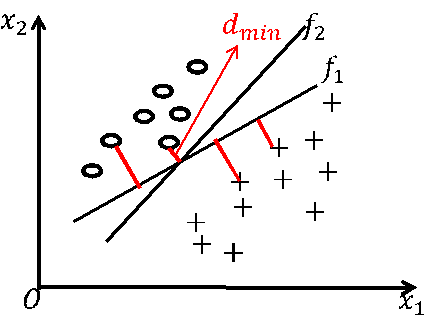
\includegraphics[height=3cm]{SVMclassify_rule1.jpg}
		\end{varwidth}
		\qquad
		\begin{varwidth}[t]{\textwidth}
		\vspace{0pt}
		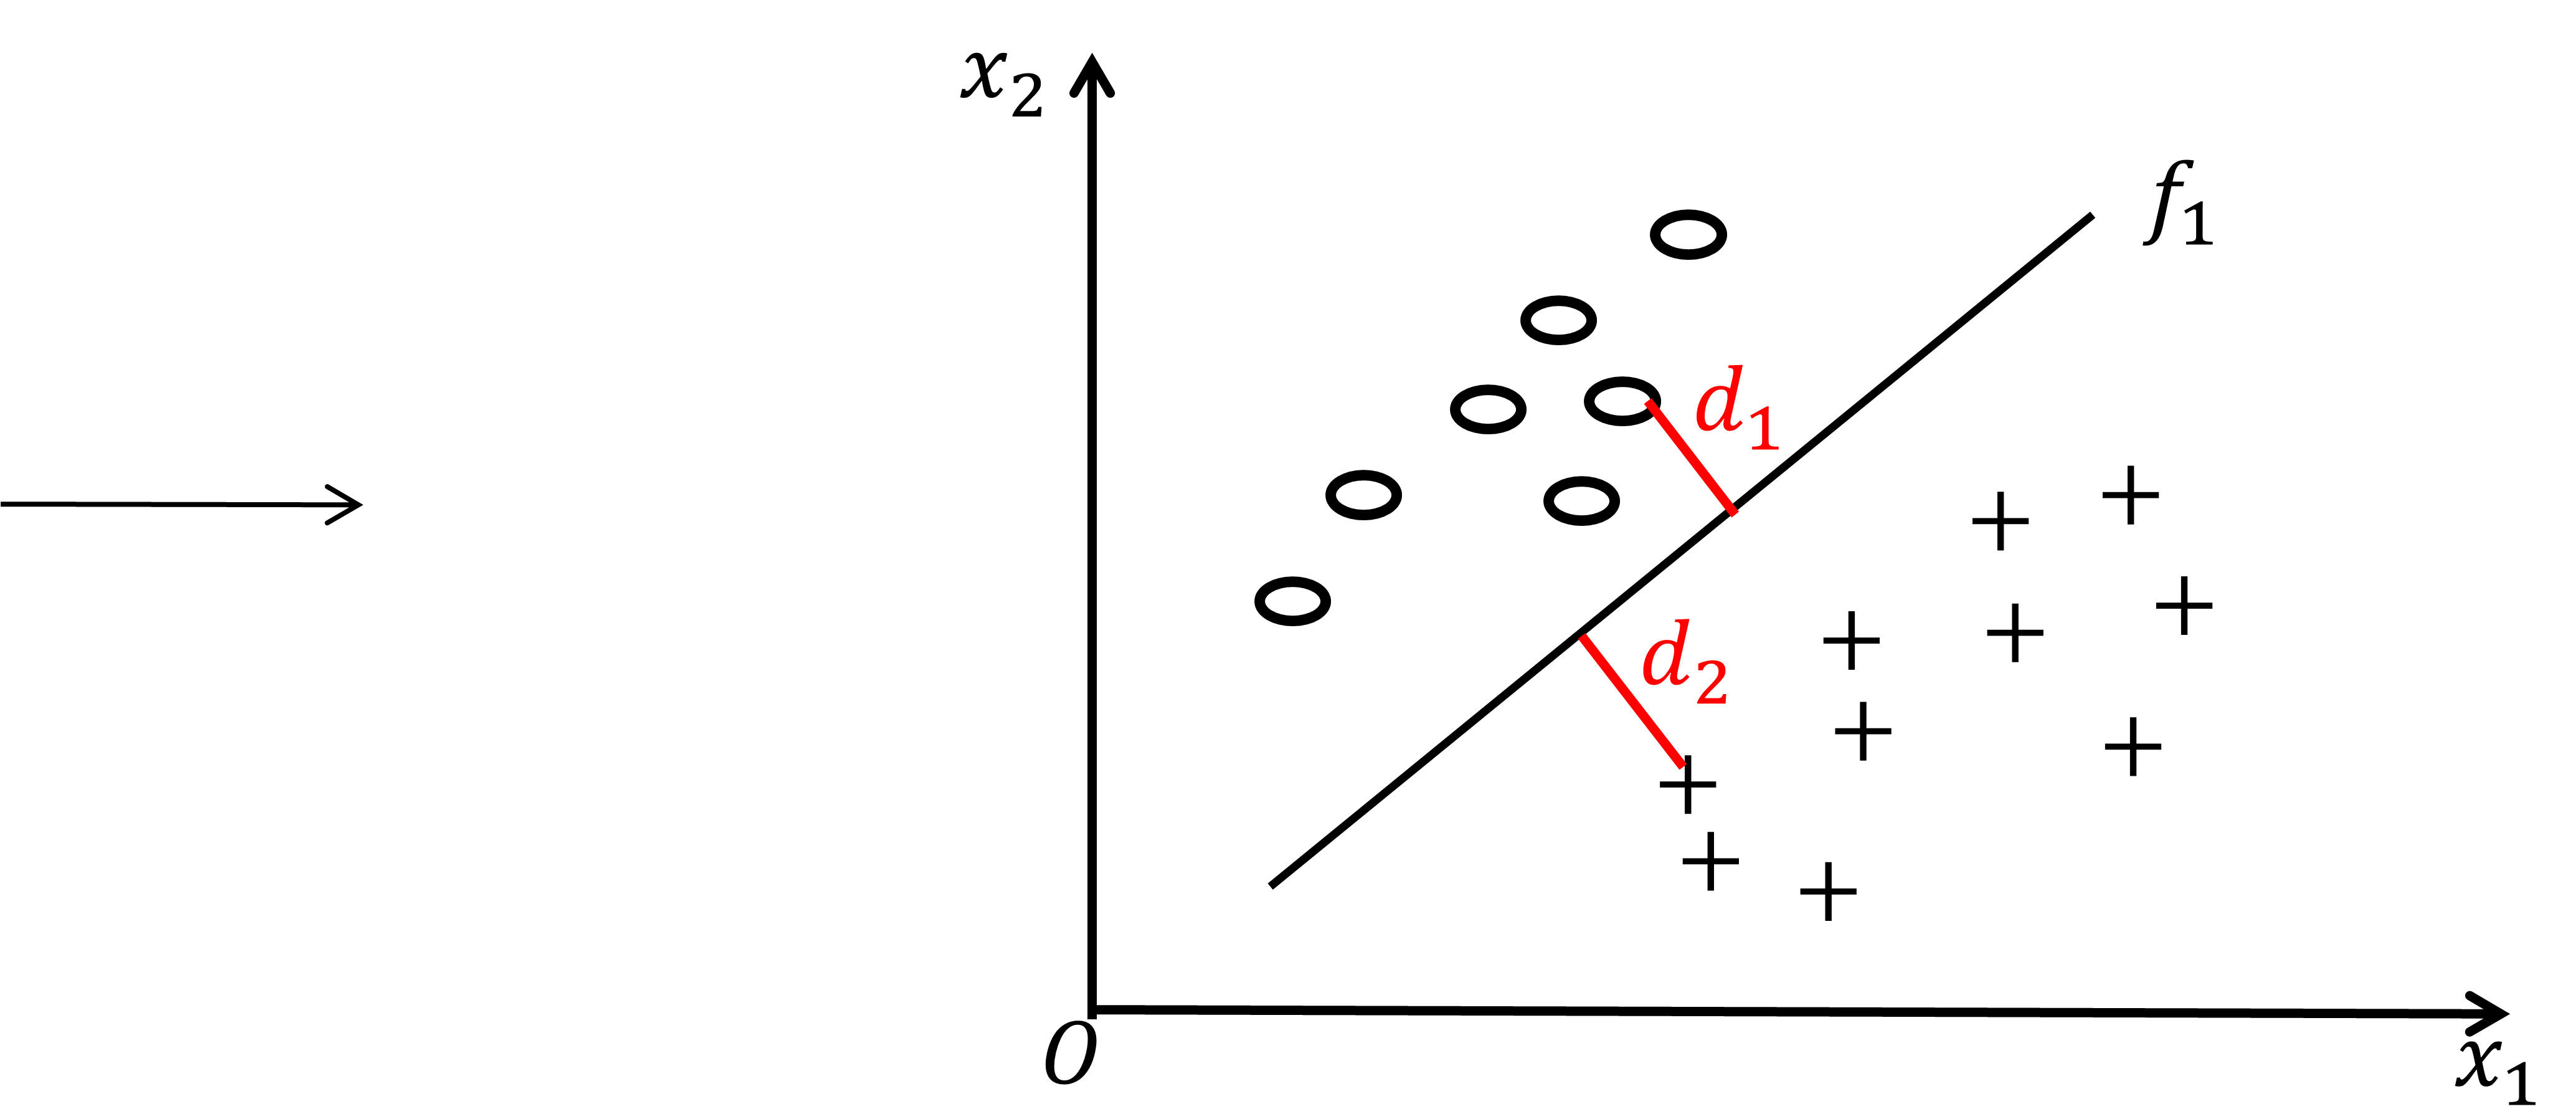
\includegraphics[height=3cm]{SVMclassify_rule2.jpg}
		\end{varwidth}
		\caption{SVM分类准则示意图}
		\label{fig:SVM分类准则示意图}
		\end{figure}
	图(\ref{fig:SVM分类准则示意图})中,我们通过平移直线$f_2$到$f_1$的位置,使得原本$f_2$的最小距离$d_{min}$尽可能大。为了书写方便,我们将第$i$个样本$x^i$写为$x_i$,记$x_i$到直线$f_1$ 的距离为
	\[
	r_i=\frac{|\mathbf w^ \mathrm{ T } x_i+b |}{||\mathbf w||}
	\]

	\par
	我们的目标是寻找$w,b$(下面的$\mathbf w$省略粗写),使得$\max \inf \{r_i\}_{i=1}^m$,也即使得两类样本点中距离直线$f_1$最近的点的距离最大,记最小距离为$d$。一定要注意的是$y=\pm1$ 要位于直线的两侧。现在,我们可以写出下面的优化模型
	\begin{gather}
	\begin{aligned}
	& \max_{w,b} \quad d \\
	& s.t. \quad \frac{|w^ \mathrm{ T } x_i+b |}{||w||}  \geqslant  d \notag \\
	\end{aligned} \\
	\forall i,j(i,j\in m) y_i=1,y_j=-1,\text 有\ (w^ \mathrm{ T } x_i+b)(w^ \mathrm{ T } x_j+b )<0 \notag
	\end{gather}
	\par
	上面的第二个约束是指:两类样本位于直线的两侧。我们将上面模型中的绝对值$|\cdot|$去掉,同时处理约束$s.t.$,可将模型转化为下面相等的优化问题
	\begin{align*}
	& \max_{w,b}\quad d \\
	& s.t.\quad \left\{
	\begin{aligned}
	& \frac{y_i(w^ \mathrm{ T } x_i+b )}{||w||}  \geqslant  d \\
	& i=1,2,\dots ,m
	\end{aligned}
	\right.
	\end{align*}
	其中:$d=\inf \{r_i\}_{i=1}^m=\frac{|w^ \mathrm{ T } x_i^*+b |}{||w||}$,$x_i^*$为距离最小的样本,即支撑向量(支持向量)。
	\par
	于是,最优化问题变为
	\begin{align*}
	&\max_{w,b}\quad \frac{|w^ \mathrm{ T } x_i^*+b |}{||w||} \\
	&s.t.\quad y_i(w^ \mathrm{ T } x_i+b )  \geqslant  |w^\mathrm{T}x_i^*+b|=y_i^*(w^ \mathrm{ T } x_i^*+b )\notag
	\end{align*}
	由于平面上距离的相对性,例如只有3个距离:$\frac {d_1}{d_2} = \frac{|w^\mathrm{T} x_1+b|}{|w^ \mathrm{T} x_2+b|}$,如图(\ref{fig:距离相对性的示意图})所示
		\begin{figure}[H]
		\centering
		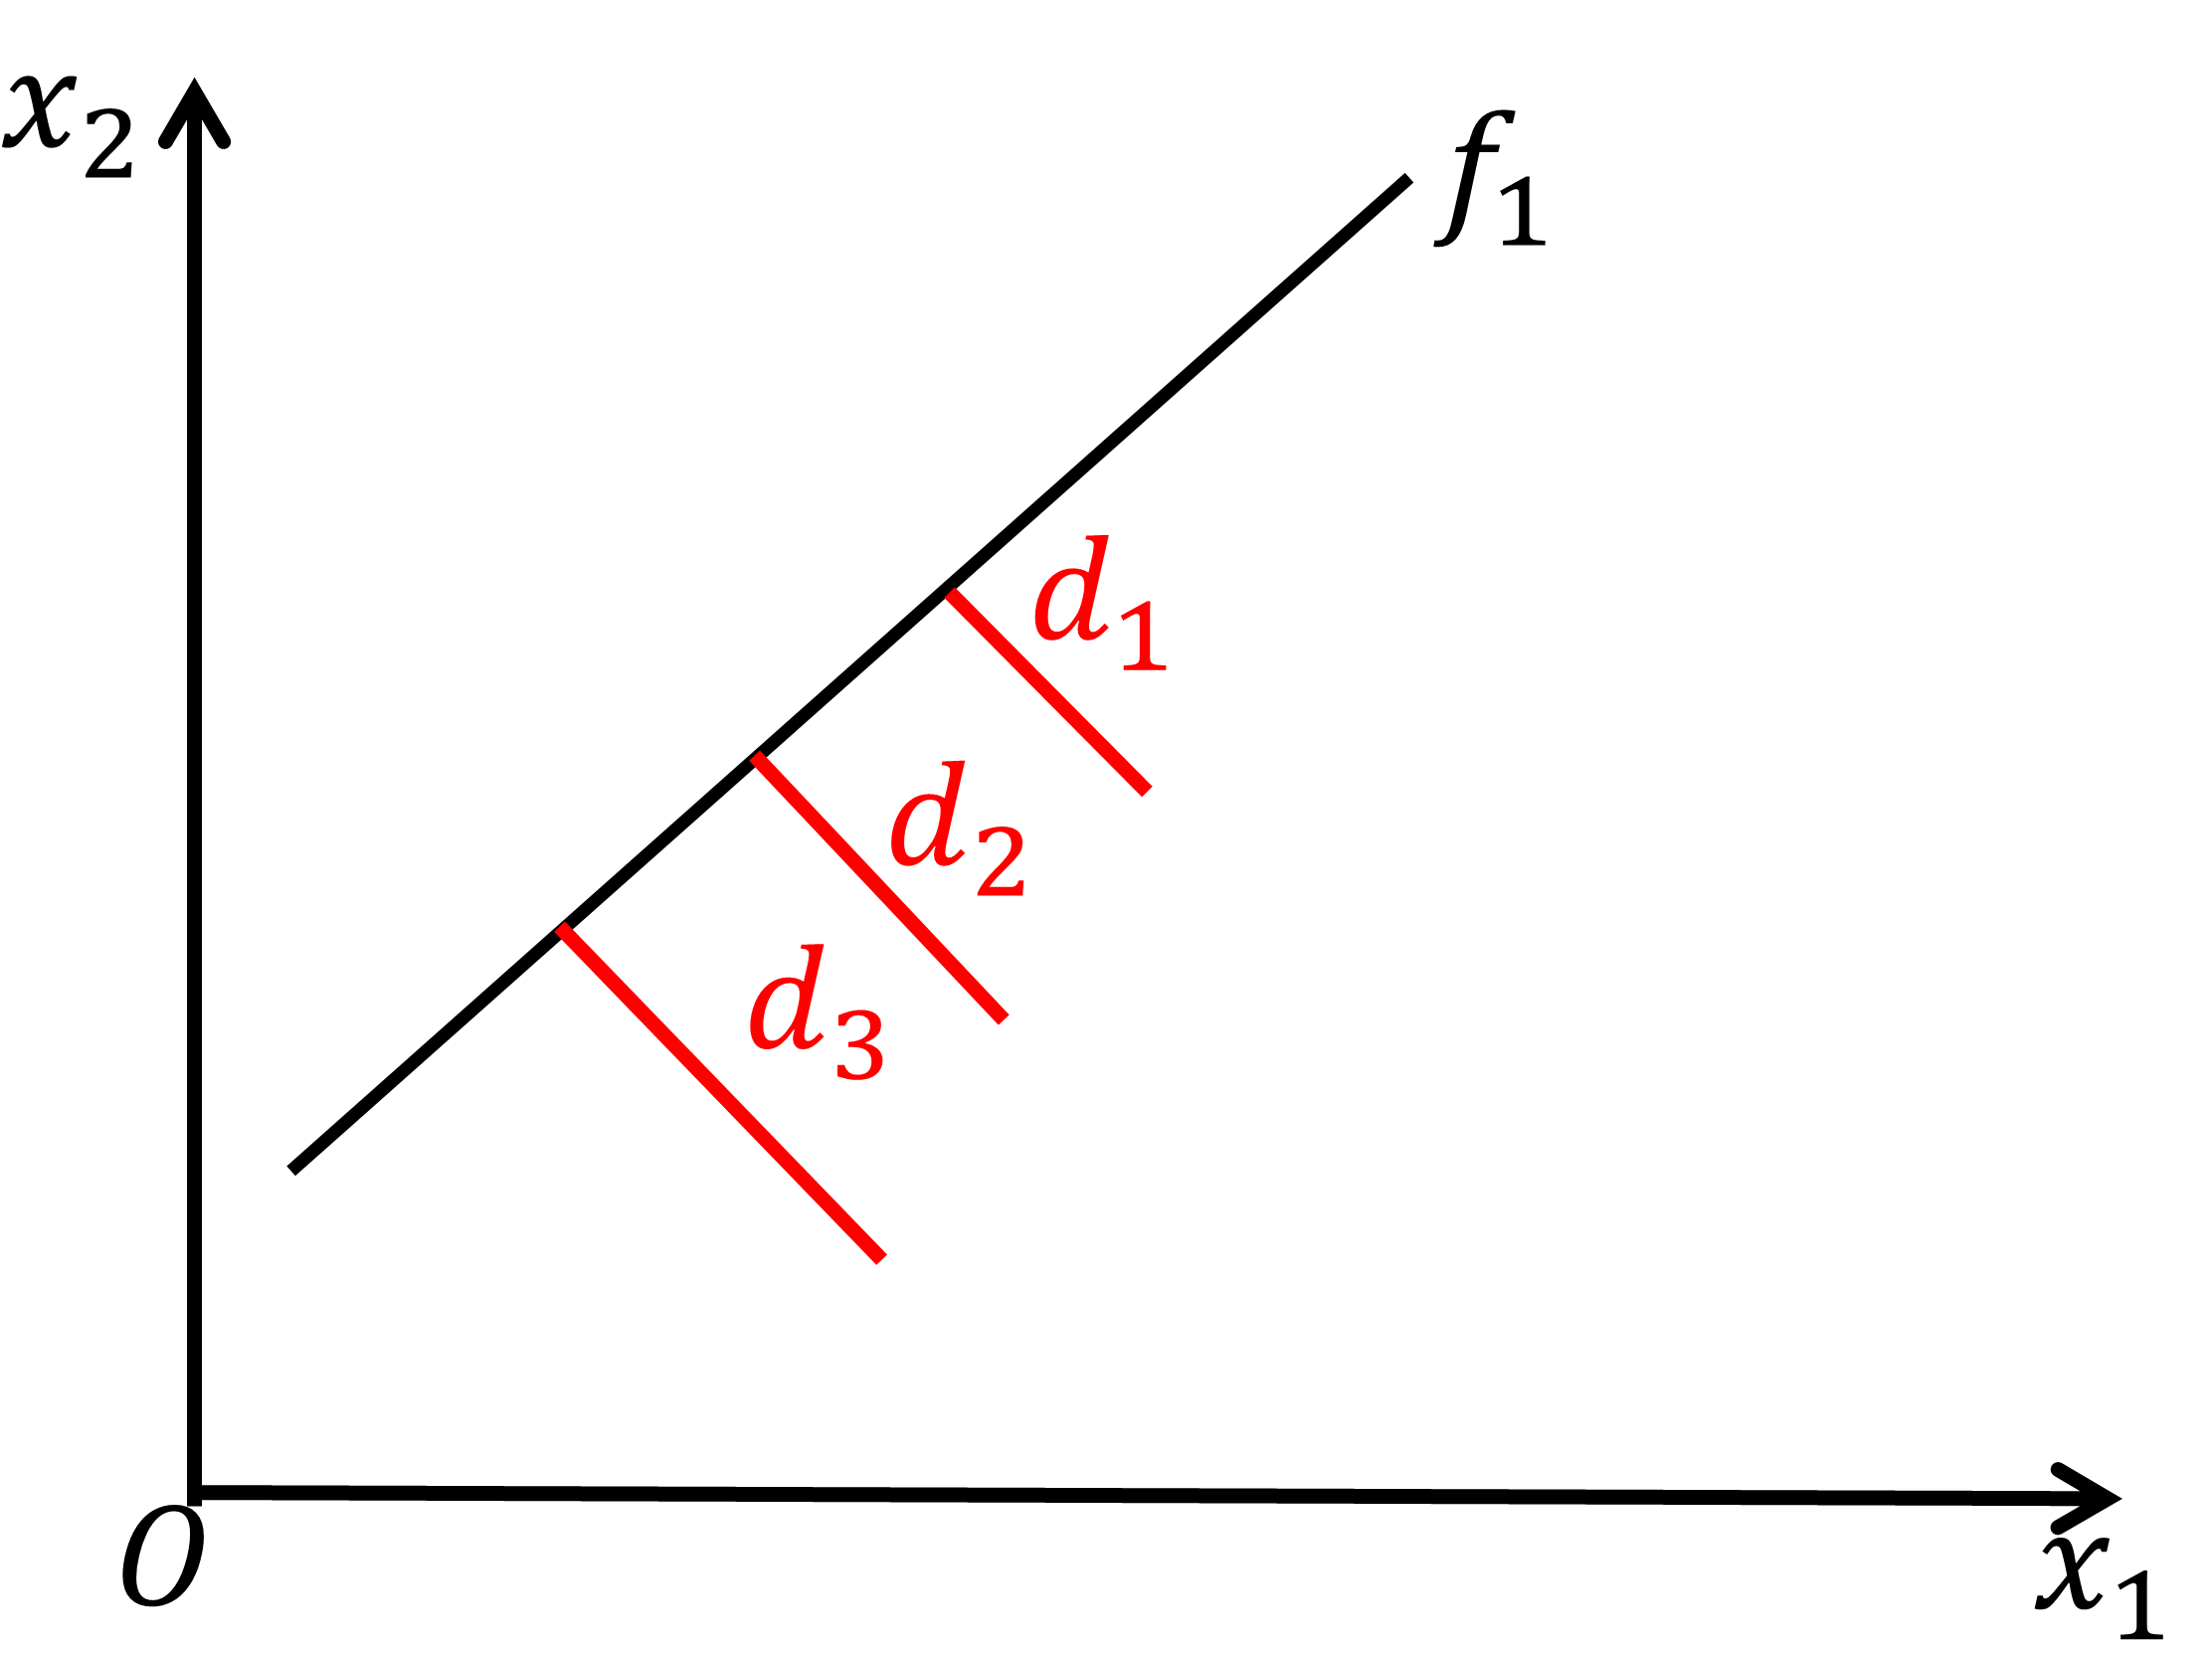
\includegraphics[width=4cm]{images/distance.jpg}
		\caption{距离相对性的示意图}
		\label{fig:距离相对性的示意图}
		\end{figure}
	不妨设$|w^\mathrm{T} x_1+b|$为\underline{元距离}$1$ (单位距离or最小距离)。于是,原优化问题变为
	\begin{align*}
	&\max_{w,b}\quad \frac{1}{||w||} \\
	&s.t.\quad y_i(w^ \mathrm{ T } x_i+b )  \geqslant  1
	\end{align*}
	注意:1、满足$(w^ \mathrm{ T } x_i+b )=1$的$x_i$即为支持向量,换句话说,支持向量记为最小距离点。2、支持向量必然是$y=\pm 1$皆有的,并且支持向量数目要大于等于2(未讨论),因为在平移直线的过程中,必然会接触另一边的点才能停止。3、解的唯一性?
	\par
	下面,我们来求解这一优化问题。按照常规的思路,用 $\mathrm{Lagrange}$对偶解法进行求解。观察上述优化问题的目标函数:$\frac{1}{||w||}=\frac{1}{\sqrt {w_1^2+w_2^2}}$,要使$\frac{1}{\sqrt{w_1^2+w_2^2}}$最大化,也即为$\sqrt{w_1^2+w_2^2}$最小化。同时,我们来处理平方$\sqrt{\cdot}$,于是,上述优化问题等价于
	\begin{align*}
	&\min_{w,b}\quad \frac{1}{2}||w||^2= \frac{1}{2}(w_1^2+w_2^2)\\
	&s.t.\quad y_i(w^ \mathrm{ T } x_i+b )  \geqslant  1\notag
	\end{align*}
	注:我们在上面的目标中添加了$\frac{1}{2}$,在后面的分析中你可以看到它的作用。
	上面的问题是一个凸二次规划问题,下面我们就来着手处理这个凸二次规划问题。

\section{凸二次规划介绍}
	% \label{sec:支持向量机-基本支持向量机-凸二次规划介绍}
	\par
	上面建立的支持向量机模型最终变为一个凸二次规划问题,下面,我们来看什么是凸集、凸函数、什么是二次规划、什么是拉格朗日对偶解法。当然,对于上面的凸二次规划问题,我们可以在原参数空间$w,b\in \Theta$上进行求解(后面,我们会给出一些求解二次规划的程序和算法),不过,如果在对偶空间(即拉格朗日乘子$\alpha\in A$)上求解,会有更神奇的效果,下面我们来逐步讨论这个神奇之处。

	\subsection{二次规划}
		\label{subsec:支持向量机-基本支持向量机-凸二次规划介绍-二次规划}
		\par
		二次规划是指如下的优化问题
		\begin{align*}
		&\max_{w}\quad \frac{1}{2} w^\mathrm{T}Hw+c^\mathrm{T}w \\
		& s.t.\quad
		\left\{
		\begin{aligned}
		& Aeq\cdot w=beq \notag\\
		& Aw \geqslant  b \notag
		\end{aligned}
		\right.
		\end{align*}
		其中:$H$为$n\times n$对称矩阵,$Aeq,A$为矩阵,$w,beq,b$为列向量。
		\par
		二次规划问题是一类特殊的非线性规划问题。如果$H$为半正定矩阵,则称此二次规划问题为凸二次规划,非凸二次规划中存在许多驻点,求解困难。常用的用于求解凸二次规划的算法有:$\mathrm{lagrange}$法、起作用集法和路径跟踪等,MATLAB中用quadprog函数进行求解。关于二次规划的具体问题,我们会在后面的章节进行详细说明。

	\subsection{凸集}
		% \label{subsec:支持向量机-基本支持向量机-凸二次规划介绍-凸集}
		\begin{definition}[凸集]
		设$S$是$R^n$中的一个集合,$S\subset R^n$,如果对$S$中的任意两点$x_1,x_2$,连接他们的线段仍属于$S$,则$S$为凸集。用数学语言描述为:$\forall x_1,x_2\in S$,$\forall \lambda \in [0,1]$,有$\lambda x_1+(1-\lambda)x_2\in S$,则$S$为凸集。
		\end{definition}
		凸集与非凸集的示意图如图(\ref{fig:凸集与非凸集的示意图})所示
		\begin{figure}[H]
		\centering
		\begin{varwidth}[t]{\textwidth}
		\vspace{0pt}
		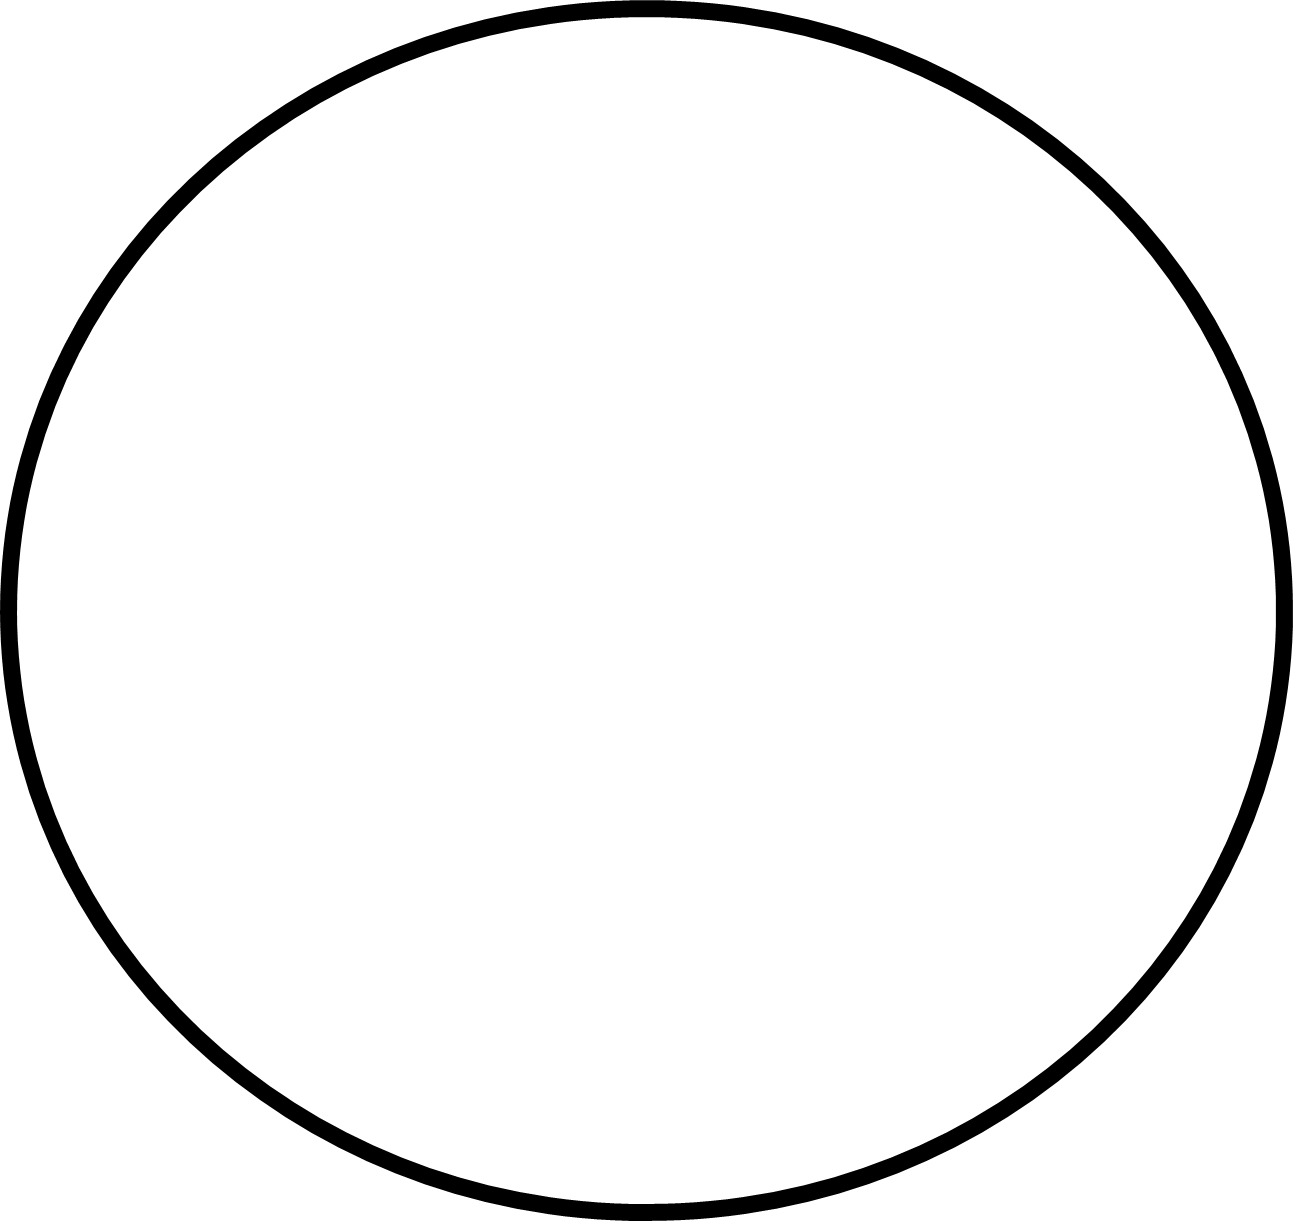
\includegraphics[height=3cm]{images/convex_set.jpg}
		\end{varwidth}
		\qquad \qquad
		\begin{varwidth}[t]{\textwidth}
		\vspace{0pt}
		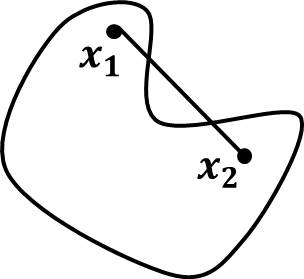
\includegraphics[height=3cm]{images/noconvex_set.jpg}
		\end{varwidth}
		\caption{凸集与非凸集的示意图}
		\label{fig:凸集与非凸集的示意图}
		\end{figure}
	\subsection{凸函数}
		% \label{subsec:支持向量机-基本支持向量机-凸二次规划介绍-凸函数}
		\par
		记得第一次接触凸函数的概念是在《数学分析讲义》刘玉琏一书中看到的,当时引入函数凸性是为了说明函数单调递增速度的问题(书上是在一元函数上进行说明的)。他给的例子是:同样是单调递增的两个函数$y=\sqrt{x}$与$y=x^2\ (x\in [0,\infty))$的增长方式不同。
		\begin{definition}[凸函数]
		设$f$在开区间$I\ I\in R^1$有定义,对$\forall x_1,x_2\in I$和$\forall \lambda\in (0,1)$,有
		\[
		f(\lambda x_1+(1-\lambda)x_2) \leqslant \lambda f(x_1)+(1-\lambda)f(x_2)
		\]
		则称函数$f$为下凸函数。
		\end{definition}
		一维下凸函数示意图如图(\ref{fig:一维下凸函数示意图})所示
		\begin{figure}[H]
		\centering
		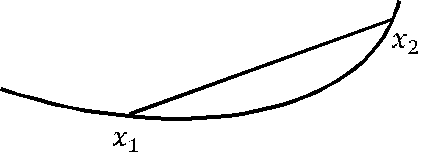
\includegraphics[width=4cm]{images/One_dimensional_convex_function.jpg}
		\caption{一维下凸函数示意图}
		\label{fig:一维下凸函数示意图}
		\end{figure}
		几何语言描述为:在$\lambda x_1+(1-\lambda)x_2$处的函数值不大于$f(x_1),f(x_2)$的加权平均$\lambda f(x_1)+(1+\lambda) f(x_2)$,即任意两点的连线在曲线的下方。
		若$f$在$I$区间是下凸的,则有Jenson不等式:
		\[
		f(q_1x_1+q_2x_2+\dots +q_nx_n) \leqslant q_1f(x_1)+q_2f(x_2)+\dots +q_nf(x_n)
		\]
		其中:$x_i\in I$,$q_i>0$,且$\sum_{i=1}^{n}q_i=1$。
		\par
		上面的凸函数是在一维情况下定义的,现在,我们将函数的凸性引入到高维空间。设$S$是$R^n$中的非空凸集,$f$是$S$上的实函数,如果$\forall x_1,x_2\in S$,$\forall \lambda\in (0,1)$,有
		\[
		f(\lambda x_1+(1-\lambda)x_2) \leqslant \lambda f(x_1)+(1-\lambda)f(x_2)
		\]
		则称函数$f$为$S$上的凸函数。
		\par
		上面给出了凸函数的定义,我们一般不能根据定义来判断函数是否为凸函数,我们只能根据凸函数的性质,找到凸函数的充分性、必要性以及充分必要性。
		\paragraph{凸函数的二阶充要条件}
		$S$是$R^n$中的非空开凸集,$f$是$S$上二次可微函数,$f$为凸函数的充要条件为:在每一个$x\in S$上,Hesse矩阵是半正定的。
		\par
		注:函数$f$在$x^*$的Hesse矩阵(Hessian Matrix)定义为
		\[
		H(x^*)=\begin{pmatrix}
		\frac{\partial ^2f(x^*)}{\partial x_1^2} & \frac{\partial ^2f(x^*)}{\partial x_1\partial x_2} & \cdots & \frac{\partial ^2f(x^*)}{\partial x_1\partial x_n} \\

		\frac{\partial ^2f(x^*)}{\partial x_2\partial x_1} & \frac{\partial ^2f(x^*)}{\partial x_2^2} & \cdots & \frac{\partial ^2f(x^*)}{\partial x_2\partial x_n} \\

		\vdots & \vdots & \ddots & \vdots\\

		\frac{\partial ^2f(x^*)}{\partial x_n\partial x_1} & \frac{\partial ^2f(x^*)}{\partial x_n\partial x_2} & \cdots & \frac{\partial ^2f(x^*)}{\partial x_n^2} \\
		\end{pmatrix}
		\]
		\par
		并且,$H$正定的充要条件是$H$左上角各阶主子式都大于0。
		\paragraph{凸函数的一阶充要条件}
		$S$是$R^n$中的非空开凸集,$f$在$S$上有一阶连续偏导数,$f$为凸函数的充要条件为:$\forall x_1,x_2\in S$,$x_1 \neq x_2$,有
		\[
		f(x_2)>f(x_1)+\nabla f(x_1)^\mathrm{T}(x_2-x_1)
		\]

	\subsection{凸规划}
		% \label{subsec:支持向量机-基本支持向量机-凸二次规划介绍-凸规划}
		\par
		上面给出了二次规划以及凸函数,下面我们来看凸规划问题(关于规划问题的详细说明,参考后面优化章节)。凸规划是一类特殊的优化问题,含约束的非线性规划问题定义如下
		\begin{align*}
		& \min_{w\in R^n}\quad f(w)\\
		& s.t. \left\{
		\begin{aligned}
		& g_i(w) \leqslant 0\quad i=1,2,\dots ,l \notag\\
		& h_j(w) = 0\quad j=1,2,\dots ,m \notag
		\end{aligned}
		\right.
		\end{align*}
		\par
		而凸规划是指$g_i$为连续可微的凸函数,$h_j$为仿射函数的规划。仿射函数是指可以用矩阵$A$和向量$b$表示成$f(w)=Aw+b$形式的函数,因为仿射矩阵有空的Hesse矩阵,因而为凸。对于前面提到过的二次规划问题,显然,当$H$为半正定时,二次规划为凸二次规划。

\section{支持向量机的求解}
	% \label{sec:支持向量机-基本支持向量机-支持向量机的求解}

	\subsection{为什么要讲凸规划}
		% \label{subsec:支持向量机-基本支持向量机-支持向量机的求解-为什么要讲凸规划}
		\par
		在求解优化问题时,我们会运用到各式各样的算法。然而,绝大多数算法可能求解的是局部最优解,而非全局最优解。那么是否有特殊类型的规划,它的局部最优解等价于全局最优解呢?后面将提到KKT条件(库恩 - 塔克)给出了算法迭代的方向:最优解必定满足KKT,但满足KKT的不一定就是最优解(即最优解仅属于KKT的子集)。但是,如果问题是凸规划问题,那么KKT条件与最优解等价(充要条件)。
		\par
		凸规划的局部最优解就是全局最优解,且极值点集合为凸集,如果凸规划的目标是严格凸,又存在极值点,那么极值点唯一。(证明可以参见《支持向量机:理论算法和拓展》P11)

	\subsection{拉格朗日对偶解法}
		% \label{subsec:支持向量机-基本支持向量机-支持向量机的求解-拉格朗日对偶解法}
		\par
		下面来考虑我们要求解的问题
		\begin{gather}
		\min_{w,b}\quad f(w)=\frac{1}{2}||w||^2= \frac{1}{2}(w_1^2+w_2^2)\\
		s.t.\quad g_i(w)=1-y_i(w^ \mathrm{ T } x_i+b ) \leqslant 0\notag
		\end{gather}
		\par
		上面,我们是在$X=(x_1,x_2)\subset R^2$上讨论的,一般的,我们可以将$X$扩展到$R^n$(共$n$个特征变量,$m$个样本),这样,待求的$w$ 变为$w\in R^n$。如果不是学习SVM,单纯的来看这个模型,会觉得很像《数学分析》里讲的条件极值问题,我们使用拉格朗日乘数法求解的条件极值问题。事实上,二者之前只差了一个符号。 如果把上面问题的$ \leqslant 0$变为$=0$ 就可以求解了。回忆一下拉格朗日乘数法:求
		\begin{align*}
		&\min_{w\in R^n}\quad f(w)\\
		&s.t.\quad h_j(w)= 0\\
		&j=1,2,\dots ,m
		\end{align*}

		解法为:\\
		1、做拉格朗日辅助函数
		\begin{align*}
		L(w,\lambda)&=f(w)+\lambda _1h_1(w)+\lambda _2h_2(w)+\dots +\lambda _mh_m(w)\\
		&=f(w)+\sum_{j=1}^m\lambda_jh_j(w)
		\end{align*}
		\par
		其中:$\lambda_j,j=1,2,\dots,m$称为拉格朗日乘子。\\
		2、求偏导,令偏导数为0,求解$w$和参数$\lambda$
		\begin{equation*}
		\left\{
		\begin{aligned}
		\frac {\partial L}{\partial w_1}&=0\\
		\vdots \\
		\frac {\partial L}{\partial w_n}&=0\\
		\end{aligned}
		\right.
		\qquad
		\left\{
		\begin{aligned}
		\frac {\partial L}{\partial \lambda_1}&=0\\
		\vdots \\
		\frac {\partial L}{\partial \lambda_m}&=0\\
		\end{aligned}
		\right.
		\end{equation*}

		\par
		上述求解过程只是针对等式约束的优化问题,并不能用于处理我们的不等式约束。下面,我们引入广义拉格朗日函数来求解如下一般形式的含不等式约束的优化问题
		\begin{align}
		\label{eq:原问题}
		& \min_{w\in R^n}\quad f(w)\\
		& s.t.\quad \left\{
		\begin{aligned}
		& g_i(w) \leqslant 0\quad i=1,2,\dots ,l \notag\\
		& h_j(w) = 0\quad j=1,2,\dots ,m \notag
		\end{aligned}
		\right.
		\end{align}
		定义广义拉格朗日函数为
		\begin{align*}
		L(w,\alpha ,\beta)=f(w)+\sum_{i=1}^l\alpha_ig_i(w)+\sum_{j=1}^m \beta_jh_j(w)
		\end{align*}
		\par
		在上面的广义拉格朗日函数的基础上,我们来求解原问题(\ref{eq:原问题})
		定义参函数$\theta(w)$(我们经常用到含参数的函数,在书中,我们都统一写为$f(x|\theta)$或者$f(x;\theta)$)
		\[
		\theta(w)=\max_{\substack{\alpha,\beta \\ \alpha_i \geqslant 0}}L(\alpha, \beta|w)
		\]
		\par
		给定某个$w$后,当$g_i(w)$或者$h_j(w)\neq 0$时,可以选取某个$\alpha_i$或者$\beta_j$,使$\alpha_i(\beta_j)\rightarrow \infty$,这样可以使$\max L(\alpha,\beta|w)\rightarrow \infty$。而当$g(w),h(w)$满足原约束$s.t.$时,$\theta(w)=f(w)$,即
		\begin{equation*}
		\centering
		\theta (w) = \left\{\begin{lgathered}
		f( w )\quad {\text{当w满足s.t.}}\\
		+ \infty \quad {\text{其他}}
		\end{lgathered} \right.
		\end{equation*}
		\par
		如果我们在此基础上考虑最小化$\theta(w)$,即$\mathop{\min}\limits_w\theta(w)$,那么,$\mathop{\min}\limits_w \theta(w)$应该完全等价于$\mathop{\min}\limits_w f(w)$,因为当$w$不满足$s.t.$时,$\theta(w) \rightarrow \infty$,这不是最小化$\min$所需要的。我们称
		\begin{equation}\label{eq:极小极大问题}
		\min_w\max_{\substack{\alpha,\beta \\ \alpha_i \geqslant 0}}L(\alpha, \beta|w)
		\end{equation}
		为广义拉格朗日函数的极小极大问题。下面,我们来分析一下这个问题:
		\par
		在$w$空间$\mathbf w$上,给定具体的某个$w_i$时,在$\alpha,\beta$空间上寻找$maxL$。姑且记其值为$L_i$,于是,每一个$w_i$都有一个$L_i$,我们找到$\min{L_i}$ 时的$w_i$即可。我们设最优解为$p^*=(\alpha,\beta,w)$,但是,我们想要求解此问题是不容易的。
		\par
		我们来定义上面极小极大问题(\ref{eq:极小极大问题})的对偶问题,可以想象着将其写出来:
		\begin{equation}\label{eq:极大极小问题}
		\max_{\substack{\alpha,\beta \\ \alpha_i \geqslant 0}}\min_wL(w|\alpha, \beta)
		\end{equation}
		\par
		没错,就是上面的形式了。我们设置其最优解为$d^*=(\alpha,\beta,w)$。我们前面说到,原始的极小极大问题(\ref{eq:极小极大问题})是不容易求解的(你可以用我们的问题进行尝试),所以,我们给出了其对偶问题(\ref{eq:极大极小问题}),此问题易解(解法后面讨论)。我们自然希望二者(\ref{eq:极小极大问题})(\ref{eq:极大极小问题})的最优解是相等的,即$d^*=p^*$,但是,事与愿违,我们来分析一下二者的大小:
		其实,对于$d^*$和$p^*$有如下关系
		\begin{equation*}
		d^*=\max_{\substack{\alpha,\beta \\ \alpha_i \geqslant 0}}\min_wL(w|\alpha, \beta) \leqslant \max_{\substack{\alpha,\beta \\ \alpha_i \geqslant 0}}\{\forall w,L(w|\alpha,\beta)\} \leqslant \min_w\max_{\alpha,\beta}L(\alpha, \beta|w)=p^*
		\end{equation*}

		即对偶问题(\ref{eq:极大极小问题})给出了原问题(\ref{eq:极小极大问题})最优解$p^*$的下界。如果不容易理解,我们可以将参数$\alpha,\beta$简化为$\theta$,于是有
		\[
		\max_\theta\min_wL(w|\theta) \leqslant \min_w\max_\theta L(\theta|w)
		\]
		\par
		上面的关系式是显然成立的,可以用一个二元函数$L(w,\theta)$进行示例。其次,从二者的名称上,我们也可以很容易理解:$\max\min \leqslant \min\max$是如此自然。也就是说,对于一般的优化问题(非凸),$d^* \leqslant p^*$,但是,值得庆幸的是,对于凸规划而言,有$d^*= p^*=(\alpha^*,\beta^*,w^*)$,即原问题与对偶问题的最优解是等价的。
		\par
		注:$\max \limits_{\substack{\alpha,\beta \\ \alpha_i \geqslant 0}}\min \limits_{ w}{L(w|\alpha, \beta)}$为凸优化问题。

	\subsection{支持向量机对偶问题}
		% \label{subsec:支持向量机-基本支持向量机-支持向量机的求解-拉格朗日对偶解法}
		\par
		上述拉格朗日对偶解法说明了:对偶问题的最优解在一定条件下可以是原问题的最优解。下面,我们对支持向量机运用拉格朗日对偶解法。\\
		1、支持向量机的原问题为
		\begin{align}
		\centering
		& \min_{w,b}\quad f(w)=\frac{1}{2}||w||^2\\
		& s.t.\quad
		\left\{
		\begin{aligned}
		& g_i(w)=1-y_i(w^ \mathrm{ T } x_i+b ) \leqslant 0 \notag\\
		& i =1,2,\dots,n \notag\\
		\end{aligned}
		\right.
		\end{align}
		注意:这里的样本量由原来的$m$变为了$n$。\\
		2、上面优化问题的广义拉格朗日函数为
		\[
		L(w,b,\alpha)=\frac{1}{2}w^\mathrm{T}w-\sum_{i=1}^n\alpha_i[y_i(w^\mathrm{T}x_i+b)-1]
		\]
		3、广义拉格朗日极小极大问题为
		\[
		\min_{w,b}\max_{\substack{\alpha \\ \alpha_i \geqslant 0}}L(\alpha|w,b)
		\]
		4、对偶问题 - 极大极小问题为
		\begin{align}\label{eq:svm的极大极小问题}
		\max_{\substack{\alpha \\ \alpha_i \geqslant 0}}\min_{w,b}L(w,b|\alpha)
		\end{align}
		\par
		为了求解(\ref{eq:svm的极大极小问题})的解$d^*$,先写$\min \limits_{w,b} L(w,b|\alpha)$,即将$\alpha$视为参数,求$L(w,b)$的最小值。用$L$对$w,b$分别求偏导,并令其为0,有
		\[
			\left\{
			\begin{aligned}
				\frac{\partial L}{\partial w} =0 \\
				\frac{\partial L}{\partial b} =0 \\
			\end{aligned}
			\right.
			\quad \text{or} \quad
			\left\{
			\begin{aligned}
				\nabla_{w}L = 0 \\
				\nabla_{b}L = 0 \\
			\end{aligned}
			\right.
		\]
		\par
		由上式推得
			\begin{equation}
			\label{eq:L求导结果}
			\centering
			\left\{\begin{lgathered}
			w-\sum_{i=1}^n\alpha_iy_ix_i=0\\
			\sum_{i=1}^n\alpha_iy_i=0\\
			\end{lgathered} \right.
			\end{equation}
		注:$x_i,y_i$为第$i$个样本,$\frac{\partial L}{\partial w} = 0$ 体现了 $ \left \| w \right \|^2$ 添加 $\frac{1}{2}$ 的优势。\\
		将(\ref{eq:L求导结果})带入$L$中,继而在$\alpha  \geqslant 0$上对其求最大值,有
		\begin{align*}
			L(w, b, \alpha)
			&= \frac{1}{2}w^\mathrm{T}w - \sum_{i=1}^{n} \alpha_i \left[ y_i(w^\mathrm{T}x_i + b) - 1 \right] \\
&= \frac{1}{2}w^\mathrm{T}w - \sum_{i=1}^{n} \alpha_i y_i w^\mathrm{T} x_i - \underset{{= 0}}{{\underline{\sum_{i=1}^{n} \alpha_i y_i b}}} + \sum_{i=1}^{n} \alpha_i \\
			&= \sum_{i=1}^{n} \alpha_i - \sum_{i=1}^{n} \alpha_i y_i w^\mathrm{T} x_i + \frac{1}{2}w^\mathrm{T} \cdot \sum_{i=1}^{n} \alpha_i y_i x_i \\
			&= \sum_{i=1}^{n} \alpha_i - \frac{1}{2} \sum_{i=1}^{n} \alpha_i y_i x_i \cdot w^\mathrm{T} \\
			&= \sum_{i=1}^{n} \alpha_i - \frac{1}{2} \sum_{i=1}^{n}\sum_{j=1}^{n} \alpha_i \alpha_j x_i x_j y_i y_j \\
			&= f(\alpha)
		\end{align*}
		\par
		于是,原SVM问题变为对偶问题(\ref{eq:SVM对偶问题})
		\begin{align}\label{eq:SVM对偶问题}
		\max_{\substack{\alpha\\ \alpha_i \geqslant 0}}\min_{w,b}L(w,b|\alpha)&=\max_{\substack{\alpha\\ \alpha_i \geqslant 0}}f(\alpha)\\
		&=\max_{\substack{\alpha\\ \alpha_i \geqslant 0}}\sum_{i=1}^n\alpha_i-\frac{1}{2}\sum_{i=1}^n\sum_{j=1}^n\alpha_i\alpha_j x_ix_jy_iy_j\notag
		\end{align}
		重新整理为
		\begin{align}
		& \max_\alpha \quad f(\alpha) =\sum_{i=1}^n\alpha_i-\frac{1}{2}\sum_{i=1}^n\sum_{j=1}^n\alpha_i\alpha_j x_ix_jy_iy_j\\
		& s.t.\quad
		\left\{
		\begin{aligned}
		& \sum_{i=1}^n \alpha_iy_i = 0 \notag \\
		& \alpha_i  \geqslant  0 \notag\\
		& i=1,2,\dots,n \notag\\
		\end{aligned}
		\right.
		\end{align}
		\par
		设上述对偶问题的最优解为$\alpha^*$,同时,注意到这个问题是一个凸二次规划问题。

	\subsection{KKT条件}
		% \label{subsec:支持向量机-基本支持向量机-支持向量机的求解-KKT条件}
		\par
		无论是前面的SVM原问题,还是上述的对偶问题,我们最终都需要求解一个非线性的凸规划问题(凸二次规划),我们下面将介绍KKT条件,来求解规划问题的最优解$d^*(\alpha,w,b)$。KKT条件用来指引我们“什么样的解可能是最优解”,这将为我们的数值计算提供方向。
		\par
		对一般的非线性规划问题
		\begin{align}
		& \min_{w\in R^n}\quad f(w)\\
		& s.t.\quad
		\left\{
		\begin{aligned}
		& g_i(w) \leqslant 0\quad i=1,2,\dots ,l \notag\\
		& h_j(w) = 0\quad j=1,2,\dots ,m \notag
		\end{aligned}
		\right.
		\end{align}
		\begin{lemma}[等式约束问题的最优解的一阶必要条件]
		$w^*$是最优解的必要条件:$\exists\beta^*$(拉格朗日乘子)当然,$w^*$必须满足等式约束条件,或者$\frac{\partial L}{\partial \lambda}=0$。使
		\end{lemma}
		\begin{align}
		\frac{\partial L}{\partial w} = \left. \frac{\partial f}{\partial w} \right|_*    + \sum_{j=1}^{m} \beta_j^* \left. \frac{\partial h}{\partial w} \right|_{w^*} = 0
		\end{align}
		\begin{lemma}[不等式约束问题的最优解的一阶必要条件(即KKT条件)]
		\begin{equation*}
		\centering
		\left\{\begin{lgathered}
		\frac{\partial f}{\partial w} + \sum_{i=1}^{l} \alpha_i \frac{\partial g}{\partial w} = 0 \\
		\alpha_i g_i (w) = 0 \\
		\alpha_i \geqslant 0
		\end{lgathered} \right.
		\end{equation*}
		当然,$w^*$必须满足不等式约束$g_i(w) \leqslant 0$。
		\end{lemma}
		\begin{lemma}[含等式和不等式约束的最优解的一阶必要条件]
		$w^*$是最优解的必要条件:$\exists\alpha^*\beta^*$,有
		\[
		\left\{
		\begin{aligned}
		& \nabla f(w) + \sum_{i=1}^{l} \alpha_i g_i(w^*) + \sum_{j=1}^{m} \beta_j h_j (w^*) = 0 \\
		& \alpha_i g_i(w) = 0 \\
		& \alpha_i \geqslant 0
		\end{aligned}
		\right.
		\]
		\end{lemma}
		注:只需用$h_i(w) \geqslant 0$和$h_i(w) \leqslant 0$替代$h_i(w)=0$进入s.t.即可。
		\par
		下面,我们来简单看一下KKT条件(在一般优化教材上都可以看到)。我们着眼于解的可行域(自变量$w$的定义域):如果$g(w)<0$,那么,我们只需要在其内求$\nabla f(w)=0$即可;如果$g(w)=0$或者$g_i(w) \leqslant 0$(即在$g(w)$可行域边界上求解),则需要进行讨论,下面我们就来看一下这种情况。
		\par
		设$w$位于第一个不等式约束的边界上(即$g_1(w)=0$),如果$w$是极小点,则$\nabla g_1(w)$必与$\nabla f(w)$在一条直线上,并且方向相反,否则,该点就存在可行下降方向,即$\exists \alpha_1 \geqslant 0$,使$\nabla f(w)+\alpha_1\nabla g_1(w)=0$。
		\par
		设$w$位于第一个不等式约束和第二个不等式约束的边界上,有$g_1(w)=0,g_2(w)=0$。如果$w$是极小点,并且$\nabla g_1(w)$与$\nabla g_2(w)$线性无关,则$\nabla f(w)$必处于$\nabla g_1(w)$与$\nabla g_2(w)$的夹角内,即$\exists \alpha_1,\alpha_2 \geqslant 0$,使
		\[
		\nabla f(w)+\alpha_1\nabla g_1(w)+\alpha_2\nabla g_2(w)=0
		\]
		递归上面的内容,有
		\[
		\nabla f(w)+\sum_{i=1}^l\alpha_i\nabla g_i(w)=0
		\]
		同时,当$g_i(w)\neq0$时,有$\alpha_i=0$;当$g_i(w)=0$时,$\alpha_i$可以不为0,于是有
		\begin{align*}
		\left\{
		\begin{aligned}
		& \alpha_i g_i (w) = 0 \\
		& \alpha_i \geqslant 0
		\end{aligned}
		\right.
		\end{align*}
		\par
		前面,我们曾经提到过,对于凸规划而言,满足KKT条件的极小点(KKT点)即为最优点,即KKT条件是最优点的充分必要条件。而且我们还提到过,对于凸规划而言,对偶问题的最优解即为原问题的最优解:
		\par
		\centerline{对偶问题的极小解$\xrightarrow[]{KKT}$对偶问题的最优解$\longrightarrow$原问题最优解}
		\par
		现在,我们可以利用KKT条件来求解SVM的对偶问题(\ref{eq:SVM对偶问题})的最优解$\alpha^*,w^*,b^*$,假设我们通过一定的算法(算法迭代的思路是依据KKT条件的,使解不断满足KKT条件)得到了$\alpha^*$,那么后面的问题是如何求$w^*,b^*$?
		\par
		$d^*=(\alpha^*,w^*,b^*)=p^*$满足KKT条件,即
		\begin{align*}
		\left\{
		\begin{aligned}
		& \nabla_w L(w^*, b^*, \alpha^*) = 0 \\
		& \nabla_b L(w^*, b^*, \alpha^*) = 0 \\
		& \alpha_i^* (y_i(w^* x_i + b^*) - 1) = 0 \\
		& y_i(w^* x_i + b^*) - 1 = 0 \\
		& \alpha_i^* \geqslant 0
		\end{aligned}
		\right.
		\end{align*}
		于是,有
		\[
		w = \sum_{i} \alpha_i y_i x_i
		\]
		其中,至少有一个$\alpha_j^*$,对此$j$,我们有
		\begin{align*}
		& y_j(w^* x_j + b^*) -1 = 0 \\
		\Rightarrow {} & y_j(\sum_{i}\alpha_i^* y_i x_i x_j + b^*) - 1 = 0 \\
		\Rightarrow {} & y_j(\sum_{i}\alpha_i^* y_i x_i x_j + b^*) = 1 =: y_j^2 \\
		\Rightarrow {} & b^* = 1 - \sum_{i}\alpha_i^* y_i x_i x_j
		\end{align*}

		\par
		至此,SVM基本的任务已经完成了,存留的问题:用算法求解对偶问题(对偶问题是一个凸二次规划)的最优解$\alpha^*$,即拉格朗日乘子,此问题后面说明。\\
		注:1、(凸)二次规划的常用解法有:块选算法、分解算法、SMO序列最优算法、起作用集法、路径跟踪法、Lemke算法等。2、$\alpha^*$中只有一些$\alpha_i^*$的值不为0,对应的是支持向量$x_i$,而且非常稀疏。

\section{容错支持向量机}
	% \label{sec:支持向量机-基本支持向量机-容错支持向量机}
	\par
	走到这里,对于一个简单的二分类问题,我们的SVM建模已经基本结束了,不过还存在一个$\alpha^*$的凸二次规划算法没有说明,这个留在后部分。虽然我们已经能够将两类样本分割开来,但这是在理想数据上进行的(即$y=\pm1$是严格线性可分的),现实中的数据情况要复杂的多。下面,我们将上面建立的模型一步步改进,让它适用于不同的问题。
	\par
	先来看一个图示的例子。在处理数据时,经常会看到异常的数据,甚至是错误的数据。还有时候会发现个别情况(特例/野点),如图(\ref{fig:分类问题异常值示意图})所示
		\begin{figure}[H]
		\centering
		\begin{varwidth}[t]{\textwidth}
		\vspace{0pt}
		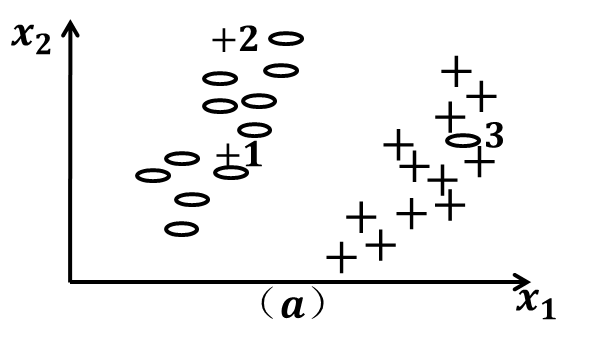
\includegraphics[height=3cm]{images/Abnormal_classification_problem1.jpg}
		\end{varwidth}
		\qquad
		\begin{varwidth}[t]{\textwidth}
		\vspace{0pt}
		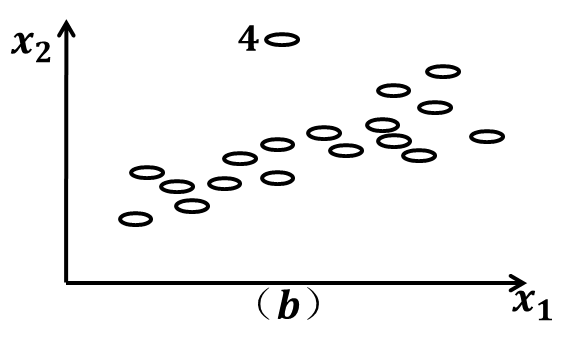
\includegraphics[height=3cm]{images/Abnormal_classification_problem2.jpg}
		\end{varwidth}
		\caption{分类问题异常值示意图}
		\label{fig:分类问题异常值示意图}
		\end{figure}
	% \textcolor[rgb]{1 0 0}{todo:图片:分类问题异常值示意图(a)(b)}
	\par
	当然,我们有专门用于挖掘奇点(1、2、3、4)的算法(SVM就可以),它们是值得研究的,但不是我们的重点。这里,我们希望能够“丢弃”这些污染,比如对于分类问题异常值示意图(a)而言,可以如图(\ref{fig:SVM处理奇点的示意图})那样来处理。我们丢弃这些污染,使得分类更加的清晰(最小距离最大化)。这也为预处理数据提供一定的思路。在使用SVM之前,可以先对异常值进行处理,如平滑数据,当然,也可以用SVM来挖掘奇点。
	\par
	先来看图(\ref{fig:SVM处理奇点的示意图})
		\begin{figure}[H]
		\centering
		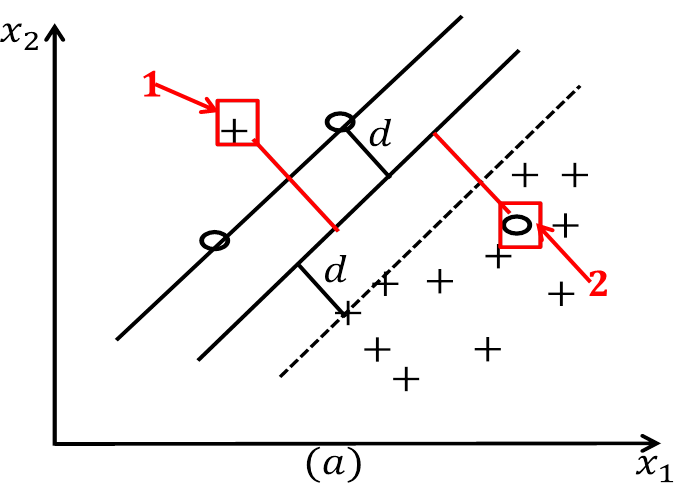
\includegraphics[width=4cm]{images/SVMdeal_with_different_point.jpg}
		\caption{SVM处理奇点的示意图}
		\label{fig:SVM处理奇点的示意图}
		\end{figure}
	在前面,我们定义了$|w^\mathrm{T}x_i^*+b|=1$,所有非支持向量(样本点)的$y_i(w^\mathrm{T}+b)>1$,但是,对于图(\ref{fig:SVM处理奇点的示意图})中的点1点2来讲,显然不是的,它们虽然不是支持向量,但是二者的$y_i(w^\mathrm{T}+b)$却是负值。为此,在其中引入松弛变量$\xi_i$,$\xi \geqslant  0$(如其名,$\xi_i$是一个变量,作用是放宽某些条件)
	\begin{align*}
	y_1(w^\mathrm{T}x_1+b)>1-\xi_1\\
	y_2(w^\mathrm{T}x_2+b)>1-\xi_2
	\end{align*}
	但是,这种“丢弃”行为会给我们造成一定的损失:\ding{172} 错判损失;\ding{173} 样本信息损失。为此,我们需要定义损失函数来控制这种损失,如果任由损失泛滥,则有可能导致如图(\ref{fig:误分现象图})的现象。\\
	% \textcolor[rgb]{1 0 0}{todo:图片:误分现象图}
		\begin{figure}[H]
		\centering
		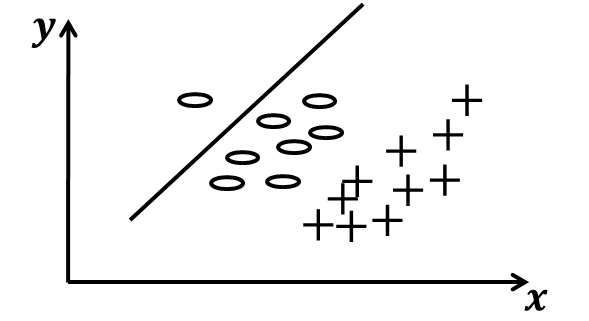
\includegraphics[width=4cm]{images/false_classify.jpg}
		\caption{误分现象图}
		\label{fig:误分现象图}
		\end{figure}
	\par
	损失函数:显然损失与$\xi_i$的大小有关,对于某点$(x_i,y_i)$而言,如果$\xi_i=0$,就不存在损失;如果$\xi_i \geqslant 0$,就存在损失;当$0<\xi_i<1$时,
	$(x_i,y_i)$样本并未被误分;当$\xi_i>1$时,样本$(x_i,y_i)$被误分,相比之下,我们更不希望这种情况的发生。令$f(\xi_i)$ 为损失函数。于是,可以设置如下极小化损失的目标
	\begin{align*}
	\min_{w,b,\xi}\quad\sum_{i=1}^n f(\xi_i)
	\end{align*}
	注:$f(\xi_i)=\xi_i,f(\xi_i)=\xi_i^2,f(\xi_i)=I(\xi_i-1)$等等,这些函数形式都可以,不过我们最好还是选取凸函数作为目标!
	\par
	将上述损失目标和原始目标(最小距离最大or分割距离最大)结合起来,可以构建如下多目标问题
	\begin{align*}
	& \max\ {\frac{1}{\left\| w \right\|}} \\
	& \min\ {\sum_{i=1}^{n}f(\xi_i)} \\
	& s.t. \left\{
	\begin{aligned}
	& y_i(w^T x_i + b) \geqslant 1 - \xi_i \\
	& \xi_i \geqslant 0 \\
	& i = 1, 2, \cdots, n
	\end{aligned}
	\right.
	\end{align*}
	\par
	将上面优化问题中的$\max$转化为$\min$,并取$f(\xi_i)=\xi_i$,用权重$c$来设置第二个目标的重要性,有
	\begin{align}
	\label{eq:容错支持向量机}
	& \min_{w,b,\xi} \quad \frac{1}{2} w^\mathrm{T} w + c \sum_{i=1}^{n} \xi_i \\
	& s.t. \quad \left\{
		\begin{aligned}
		& y_i(w^\mathrm{T} x_i + b) \geqslant 1 - \xi \notag\\
		& \xi_i \geqslant 0 \notag\\
		& i = 1,2,\cdots,n \notag\\
		\end{aligned}
	\right.
	\end{align}
	\par
	容错支持向量机的模型已经建好了,就是在原SVM模型上进行改进的,注意,上面的模型仍然是一个凸二次规划问题,我们可以依据前面的思路,对其进行拉格朗日对偶求解。在此之前,值得一提的是:目标中的第二项$\sum_{i=1}^n\xi_i$在统计学习理论中叫做经验风险,广义上可以记为$\Omega (f)$,第一项$w^\mathrm{T}w$叫做结构风险。在统计学习理论中,有许多最优超平面(即高维的分割面)的性质和定理,这里不多做说明,可以参考《统计学习理论》Vapnilk一书。下面,我们来求解
	(\ref{eq:容错支持向量机})模型,限于篇幅,这里不做展开,直接给出其对偶问题
	\begin{align}
	\label{eq:容错支持向量机对偶模型}
	& \max_{\alpha} \quad \sum_{i=1}^{n} \alpha_i - \frac{1}{2}\sum_{i=1}^{n}\sum_{i=1}^{n}\alpha_i \alpha_j y_i y_j x_i x_j \\
	& s.t. \quad \left\{
		\begin{aligned}
		& \sum_{i=1}^{n} \alpha_i y_i = 0 \notag\\
		& 0 \leqslant \alpha_i \leqslant c \notag\\
		& i = 1,2,\cdots,n \notag\\
		\end{aligned}
	\right.
	\end{align}
	\par
	将上述模型(\ref{eq:容错支持向量机对偶模型})写为矩阵形式,且转化为最小化问题,有
	\begin{align}\label{eq:容错支持向量机对偶模型矩阵形式}
	& \min_{\alpha} \quad \frac{1}{2}\alpha^T Q \alpha - e^T \alpha \\
	& s.t. \quad \left\{
		\begin{aligned}
		& y^T \alpha = 0 \notag\\
		& 0 \leqslant \alpha_i \leqslant c \quad or \quad 0 \leqslant \alpha \leqslant ce \notag\\
		\end{aligned}
	\right.
	\end{align}
	\noindent
	其中:$e$是全1向量,$Q$是对称矩阵,$Q_{ij}=y_iy_jx_ix_j$
	\par
	上述问题仍是一个凸规划问题,其求解方式仍然在后面的章节。我们姑且称上述容错二分类支持向量机为C-SVM。\\
	注:如何确定外来参数$c$:CV方法或者(智能)优化;能否在原参数空间上求解C-SVM?

\section{核技术的引入}
	% \label{sec:支持向量机-基本支持向量机-核技术的引入}
	\par
	上面建立的C-SVM使得我们可以处理一些非完全线性可分数据,但是,在实际工作中,要求绝不会如此简单,有许多非线性问题等待我们讨论,比如下面这些图中的问题,非线性可分如图(\ref{fig:非线性可分示意图})所示
		\begin{figure}[H]
		\centering
		\begin{varwidth}[t]{\textwidth}
		\vspace{0pt}
		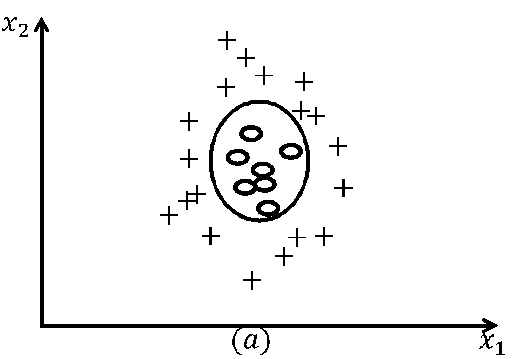
\includegraphics[height=4cm]{images/Nonlinear_classify1.jpg}
		\end{varwidth}
		\qquad \qquad
		\begin{varwidth}[t]{\textwidth}
		\vspace{0pt}
		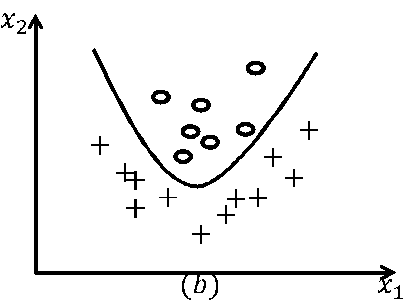
\includegraphics[height=4cm]{images/Nonlinear_classify2.jpg}
		\end{varwidth}
		\caption{非线性可分示意图}
		\label{fig:非线性可分示意图}
		\end{figure}
	% \textcolor[rgb]{1 0 0}{todo:图片:非线性可分示意图(a)(b)} \\
	如果存在某些奇点(干扰点/野点/离群点),会有非线性非完全可分问题,如图(\ref{fig:非线性非完全可分示意图})的情况
		\begin{figure}[H]
		\centering
		\begin{varwidth}[t]{\textwidth}
		\vspace{0pt}
		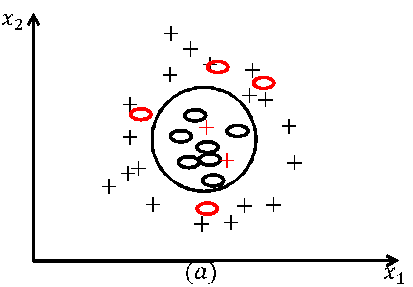
\includegraphics[height=4cm]{images/Nonlinear_nocomplete_classify1.jpg}
		\end{varwidth}
		\qquad \qquad
		\begin{varwidth}[t]{\textwidth}
		\vspace{0pt}
		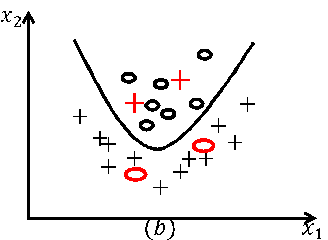
\includegraphics[height=4cm]{images/Nonlinear_nocomplete_classify2.jpg}
		\end{varwidth}
		\caption{非线性非完全可分示意图}
		\label{fig:非线性非完全可分示意图}
		\end{figure}
	图(\ref{fig:非线性非完全可分示意图})的情况是在图(\ref{fig:非线性可分示意图})上引入松弛变量$\xi$的情况,我们来看一下图(\ref{fig:非线性可分示意图})中的分类器:
	\begin{itemize}
	  \item 图(\ref{fig:非线性可分示意图})(a)的分类线为:$(x_1-a)^2+(x_2-b)^2=r^2$;
	  \item 图(\ref{fig:非线性可分示意图})(b)的分类线为:$x_2=ax_1^2+bx_1+c$;
	\end{itemize}
	\par
	上面两个分类线都是$x_1Ox_2$中的非线性函数,将$(x_1-a)^2+(x_2-b)^2=r^2$变形,有
	\begin{align}\label{eq:非线性分类器1}
	x_1^2-2ax_1+x_2^2-2bx_2+a^2+b^2-r^2=0
	\end{align}
	也即
	\begin{align}\label{eq:非线性分类器2}
	w_1x_1^2+w_2x_1+w_3x_2^2+w_4x_2+b=0
	\end{align}
	可以看出,非线性分类线(\ref{eq:非线性分类器1})虽然不是$x_1,x_2$的线性函数,但却是它们变形后$(x_1,x_1^2,x_2,x_2^2)$的线性函数(\ref{eq:非线性分类器2})。
	\par
	我们称$X=(x_1,x_2)\subset R^2$为原始特征空间,称$X^*=(x_1,x_1^2,x_2,x_2^2)\subset R^4$是变换后的新特征空间。我们可以定义一个变化$\phi(\cdot)$,$\phi(\cdot)$使得$X$变为$X^*$
	\[
	\phi(X)=X^*
	\]
	\par
	从数据上看,$\phi(\cdot)$的作用是这样的
	\begin{equation*}
	\begin{matrix}
	x_1 & x_2 \\
	\vdots & \vdots \\
	\end{matrix}
	\quad \underrightarrow{\phi(\cdot)} \quad
	\begin{matrix}
	x_1 & x_1^2 & x_2 & x_2^2 \\
	\vdots & \vdots & \vdots & \vdots \\
	\end{matrix}
	\end{equation*}
	\par
	就上面的问题而言,在变换后的新空间上建立线性的C-SVM就可以解决这个非线性分类问题。但一般而言,我们并不知道新特征空间的形式(即$X$变换后的$X^*$中只有$x_1,x_1^2,x_2,x_2^2$),那么该如何确定转换$\phi(\cdot)$呢?
	\par
	想一个复杂的变换:我们将所有可能的情况都列举出来
	\begin{equation}
	(x_1, x_2) \longrightarrow (x_1 x_1^2 x_1^3 \cdots x_1^l, \, x_2 x_2^2 x_2^3 \cdots x_2^l, \, x_1 x_2 x_1^2 x_2 \cdots)_{l \rightarrow \infty}
	\label{eq:完整变换phi}
	\end{equation}
	\par
	当不存在上面变换后的某项时,我们令其权重$w$为0即可。可是,如果像上式(\ref{eq:完整变换phi})那样来处理$\phi(\cdot)$,会给我们的处理以及计算带来很多麻烦,而且还要限定一些外来参数$l$。为了解决这个问题,我们引入核函数这个工具,在此之前,我们来看一下前面C-SVM的分类线(如果$X\subset R^n$,则称分类线为分类超平面)。
	\[
	w^*x+b^*=0
	\]
	其中:$x\in R^2$,$w^*=\sum_{i=1}^n\alpha_i^*y_ix_i$,所以,上式又可以写为
	\[
	\sum_{i=1}^n\alpha_i^*y_ix_ix+b=0
	\]
	\par
	上式中除了有$x$外,还有$x_ix$,如此看来,我们除了要关心变换$\phi(\cdot)$以外,还要关心$\phi(x_i)\phi(x)$。
	\begin{definition}[核函数]
	设$X$是原特征空间($X\subset R^n$),设$H$是新的特征空间($H$是Hilber空间:Hilber空间可以看作$n$维欧式空间的无穷维推广),如果存在一个从$X\rightarrow H$的映射
	\[
	\phi(X):X\rightarrow H
	\]
	使得对于所有的$x_i,x_j(x_i,x_j\in X\subset R^n)$,有函数$K(x_i,x_j)$
	\[
	K(x_i,x_j)=\phi(x_i)\phi(x_j)
	\]
	则称函数$K(x_i,x_j)$为核函数。其中:$\phi(x_i)\phi(x)$表示内积,所以$K$亦被称为内积核函数。
	\end{definition}
	注:对于给定的核函数$K$,$H$和$\phi$二者的取法不唯一;内积核函数为对称核函数:$K(x_i,x_j)=K(x_j,x_i)$;核函数$K(x,y)$是定义在$R^n\times R^n$上的函数,即$x_i,x_j\in X\subset R^n$。
	\par
	前面,提问过该如何确定$\phi(\cdot)$?其实,$\phi(\cdot)$在未分类之前(分类器SVM未构建之前)是不能确定的,我们只能假设它是某种形式,例如:可以将其假设为$\phi(X)=(x_1,x_2,x_1x_2)$,也可以假设为$\phi(X)=(x_1,x_2^2,x_1x_2^2)$ 等等形式,当然也可以像前面的“最复杂的变换”
	式(\ref{eq:完整变换phi})。这种做法的本质目的是将原始特征空间$X$引入到新的高维特征空间。前面说过即便给定了$K(\cdot)$,其映射变换$\phi(\cdot)$也是不确定的。而$\phi(\cdot)$本身就是我们假设的(本身即不确定),所以可以跳过$\phi(\cdot)$而直接假设$K(\cdot)$的形状。$K(\cdot)$的作用仍就是将原始空间投影到高维空间。值得一提的是:并不是$K(\cdot)$或者$\phi(\cdot)$的形式越复杂越好,像前面提到的“最复杂的变换”,即上式(\ref{eq:完整变换phi}),因为那样会出现过拟合现象。
	\par
	我们可以来事先假设内积核函数$K(\cdot)$的形状,但是什么样的函数是内积核函数呢?Mercer 定理给了我们答案。
	\begin{theorem}[Mercer定理]
	任何半正定的函数都可以作为核函数。其实内积核函数$K(x_i,x_j)$($x_i,x_j\in X\subset R^n$)是泛函分析中Mercer定理的一种特殊形式。如果$K(x_i,x_j)$是定义在$X\times X$$\left(L_2(X)\right)$上的连续对称函数,其中,$X$是$R^n$的紧集,且有$\int_X\int_X K(x_i,x_j)g(x_i)g(x_j)\mathrm{d}x_i\mathrm{d}x_j \geqslant 0$ 成立$\left(\forall g\in L_2(X)\right)$,则$\exists\phi(\cdot)$,使得$K(x_i,x_j)=\phi(x_i)\phi(x_j)$,反之亦成立。
	\end{theorem}
	\par
	Mercer定理可以帮助我们判断一个函数$K(\cdot)$是否可以作为核函数,如果是核函数,那么就可以将其运用到SVM中。下面给出一些常用的核函数,至于如何构建核函数,这里就不做讨论了。常见的核函数如表(\ref{tab:支持向量机-基本支持向量机-常见的核函数})所示
	\begin{table}[H]
		\caption{常见的核函数}
		\label{tab:支持向量机-基本支持向量机-常见的核函数}
		\centering
		\begin{tabular}{ll}
		\toprule
		核函数 & 表达式 \\
		\midrule
		线性核:& $ k(x_i y_i) = x_i \cdot y_i $ \\
		多项式核:& $ k(x_i y_i) = (\gamma x_i \cdot y_i + r)^d \quad d \geqslant 1 \quad \gamma > 0 $ \\
		高斯核:& $ k(x_i y_i) = \exp (-\frac{\| x_i - y_i \|^2}{2 \sigma^2}) \quad \sigma > 0 $ \\
		RBF 核:& $ k(x_i y_i) = \exp (-\gamma \| x_i - y_i \|^2) \quad \gamma > 0 $ \\
		B 样条核:& $ k(x_i y_i) = B_{2N+1} \left( \left\| x_i - y_i \right\| \right) $ \\
		sigmoid 核:& $ k(x_i y_i) = \tanh(x_i \cdot y_i + r) \quad \tanh(x) = \frac{ e^x }{ e_x + 1 } \quad \gamma > 0 \quad r<0 $ \\
		拉普拉斯核:& $ k(x_i y_i) = \exp(-\frac{ 1 }{ 6 } \left\| x_i - y_i \right\| ) \quad \sigma > 0 $ \\
		小波核:& \\
		混合核:& \\
		\bottomrule
		\end{tabular}
	\end{table}
	\par
	\paragraph{核函数的性质}如果$K_1$和$K_2$是$X\times X$$\left(L_2(X)\right)$上的核函数,则$\alpha K(\alpha \geqslant 0)$,$K_1+K_2$和$K_1\cdot K_2$也是核函数。并且$\forall g$,$g(x)k(x,y)g(y)$亦为核函数。\\
	那么问题来了:
	\begin{itemize}
	  \item 这么多的核函数,如何选择适合的核函数呢?评价标准是什么?
	  \item 核函数中有一些外来的参数$\gamma$等等,如何确定这些参数?
	\end{itemize}
	注:关于正定核,我们没有讨论,设$K$是$L_2(X)$上的对称函数,$K$为正定核的充要条件是:对$\forall x_i\in X(i=1,2,\dots,n)$,$K$对应的矩阵$\mathbf K=\left[K(x_i,x_j)\right]$ ,$\mathbf K_{ij}=K(x_i,x_j)$是半正定的。Mercer核是正定核,多项式核、高斯核也是正定核。
	\par
	现在,可以将核函数$K$引入到前面的C-SVM中,使C-SVM可以处理非线性分类情况。设我们假设的(挑选的)核函数为$K$,其变换(映射)为$\phi$。对于C-SVM,有
	\begin{align*}
	& \min_{w,b,x} \ \frac{1}{2} w^T w + c \cdot \sum_{i=1}^{n} \xi \\
	& s.t. \left\{
	\begin{aligned}
	& y_i (w^T \phi (x_i) + b) \geqslant 1 - \xi_i \\
	& \xi \geqslant 0 \\
	& i = 1,2,\cdots,n
	\end{aligned}
	\right.
	\end{align*}
	其对应的对偶问题(写成min形式)为:
	\begin{align*}
	& \min_\alpha \ \frac{1}{2} \sum_{i=1}^{n} \sum_{j=1}^{n} \alpha_i \, \alpha_j \, y_i \, y_j \, k(x_i y_i) - \sum_{i=1}^{n} \alpha_i \\
	& s.t. \left\{
	\begin{aligned}
	& \sum_{i=1}^{n} \alpha_i \,  y_i = 0 \\
	& 0 \leqslant \alpha_i \leqslant c \\
	& i = 1, 2, \cdots, n
	\end{aligned}
	\right.
	\end{align*}
	\par
	至此,支持向量机模型已经基本构建完毕,后面的工作是对C-SVM的性能的讨论以及模型的变换与改进。关于SVM的性能我们可以讨论其优化模型的求解算法,模型中参数的选取以及核函数的性质等诸多方面。而关于SVM的变种与派生更是数不胜数。
	\par
	在讨论SVM的性能之前,我们先来看一个小例子\footnote{《神经网络原理》SimonHaykin著,叶世伟译P241},这个例子可以更好地帮助我们理解SVM。

\section{SVM解决xor问题的小例子}
	% \label{sec:支持向量机-基本支持向量机-SVM解决xor问题的小例子}
	给出原始数据 data
	\[
	\begin{matrix}
		x_1 & x_2 & y \\
		-1 & -1 & -1 \\
		-1 & +1 & +1 \\
		+1 & -1 & +1 \\
		+1 & +1 & -1 \\
	\end{matrix}
	\]
	为了进行分割,先给出核函数 $K$,选定的核函数为
	\begin{align*}
		K(x_i, y_i) &= (1 + x_i y_i)^2 \\
				   &= 1 + x_{i1}^2 x_{j1}^2 + 2 x_{i1}x_{i2}x_{j1}x_{j2} + x_{i2}^2 x_{j2}^2 + 2x_{i1}x_{j1}^2 + 2x_{i2}x_{j2}
	\end{align*}
	可以写出 $K$ 在 $H$ 为 6 时的 $ \phi(x) $
	\[
	\phi(x_i) = \left[ 1, \, x_{i1}^2, \, \sqrt{2} x_{i1}x_{i2}, \, x_{i2}^2, \, \sqrt{2}x_{i1}, \, \sqrt{2}x_{i2}  \right]^T
	\]
	可以写出 $K$ 在 $ \alpha_i \, (i=1,2,3,4) $ 上对应的 $\mathrm{Gram}$ 矩阵 $\mathbf{K}_{ij}$ \\
	\begin{align*}
	\mathbf{K} =
	\begin{bmatrix}
		q & 1 & 1 & 1 \\
		1 & q & 1 & 1 \\
		1 & 1 & q & 1 \\
		1 & 1 & 1 & q \\
	\end{bmatrix}
	\end{align*}
	$ SVM $ 的对偶问题为
	\begin{align*}
	& \max_{\alpha} \quad \alpha_1 + \alpha_2 + \alpha_3 + \alpha_4 - \frac{1}{2} (9 \alpha_1^2 - 2 \alpha_1 \alpha_2 \\
	& \qquad \qquad -2 \alpha_1 \alpha_3 + 2 \alpha_1 \alpha_4 + 9 \alpha_2^2 + 2 \alpha_2 \alpha_3 -2 \alpha_2 \alpha_4 + 9 \alpha_3 \alpha_4 + 9 \alpha_4^2 ) \\
	& s.t. \quad \left\{
	\begin{aligned}
	& \sum_{i=1}^{n} \alpha_i y_i = 0 \\
	& 0 \leqslant \alpha_i \\
	& i = 1,2,3,4
	\end{aligned}
	\right.
	\end{align*}
	对 $ \mathrm{Lagrange} $ 乘子优化产生下列方程组
	\begin{align*}
	\left\{
	\begin{aligned}
	&9 \alpha_1 - \alpha_2   - \alpha_3   + \alpha_4   = 1 \\
	&-\alpha_1  + 9 \alpha_2 + \alpha_3   - \alpha_4   = 1 \\
	&-\alpha_1  + \alpha_2   + 9 \alpha_3 - \alpha_4   = 1 \\
	&\alpha_1   - \alpha_2   - \alpha_3   + 9 \alpha_4 = 1 \\
	\end{aligned}
	\right.
	\end{align*}
	因此,$ \mathrm{Lagrange} $ 乘子 $\alpha$ 的最优值 $\alpha^*$ 为
	\[
	\alpha_1 = \alpha_2 = \alpha_3 = \alpha_4 = \frac{1}{8}
	\]
	说明数据中的 4 个向量皆为支持向量,目标函数最优值为 $\frac{1}{4} $,
	最优权重 $w^*$ 为
	\begin{align*}
	w^* &= \sum_{i=1}^{n} \alpha^* y_i \cdot \varphi (x_i) \\
	    &= \frac{1}{8} \left[ -\varphi(x_1) + \varphi(x_2) + \varphi(x_3) - \varphi(x_4) \right] \\
	    &= \frac{1}{8} \left[
	    - \begin{bmatrix}
	    1 \\
	    1 \\
	    \sqrt{2} \\
	    1 \\
	    -\sqrt{2} \\
	    -\sqrt{2} \\
	    \end{bmatrix}
	    + \begin{bmatrix}
	    1 \\
	    1 \\
	    -\sqrt{2} \\
	    1 \\
	    -\sqrt{2} \\
	    \sqrt{2} \\
	    \end{bmatrix}
	    + \begin{bmatrix}
	    1 \\
	    1 \\
	    -\sqrt{2} \\
	    1 \\
	    \sqrt{2} \\
	    -\sqrt{2} \\
	    \end{bmatrix}
	    - \begin{bmatrix}
	    1 \\
	    1 \\
	    \sqrt{2} \\
	    1 \\
	    \sqrt{2} \\
	    \sqrt{2} \\
	    \end{bmatrix}
	    \right] \\
	    &= \begin{bmatrix}
	    0 \\
	    0 \\
	    -\frac{1}{\sqrt{2}} \\
	    0 \\
	    0 \\
	    0 \\
	    \end{bmatrix}
	\end{align*}
	最优偏量 $b^*$ 为 $w$ 的第一个分量为 $0$ 。
	\par
	最优超平面为
	\begin{align*}
	 w^* \cdot \varphi(x) &= 0 \\
	 \left[ 0,0,-\frac{1}{\sqrt{2}},0,0,0 \right] \,
	\begin{bmatrix}
	1 \\
	x_1^2 \\
	\sqrt{2} x_1 x_2 \\
	x_2^2 \\
	\sqrt{2} x_1 \\
	\sqrt{2} x_2
	\end{bmatrix}
	&= 0
	\end{align*}
	即 $-x_1 x_2$ = 0 。
	\par
	决策函数(分类线)为
	\begin{align*}
	f(x) &= \mathrm{sgn} \, (w^* \cdot \varphi(x)) \\
	     &= \mathrm{sgn} \, (-x_1 x_2)
	\end{align*}




% \end{document}
